% Options for packages loaded elsewhere
\PassOptionsToPackage{unicode}{hyperref}
\PassOptionsToPackage{hyphens}{url}
%
\documentclass[
]{article}
\usepackage{amsmath,amssymb}
\usepackage{iftex}
\ifPDFTeX
  \usepackage[T1]{fontenc}
  \usepackage[utf8]{inputenc}
  \usepackage{textcomp} % provide euro and other symbols
\else % if luatex or xetex
  \usepackage{unicode-math} % this also loads fontspec
  \defaultfontfeatures{Scale=MatchLowercase}
  \defaultfontfeatures[\rmfamily]{Ligatures=TeX,Scale=1}
\fi
\usepackage{lmodern}
\ifPDFTeX\else
  % xetex/luatex font selection
\fi
% Use upquote if available, for straight quotes in verbatim environments
\IfFileExists{upquote.sty}{\usepackage{upquote}}{}
\IfFileExists{microtype.sty}{% use microtype if available
  \usepackage[]{microtype}
  \UseMicrotypeSet[protrusion]{basicmath} % disable protrusion for tt fonts
}{}
\makeatletter
\@ifundefined{KOMAClassName}{% if non-KOMA class
  \IfFileExists{parskip.sty}{%
    \usepackage{parskip}
  }{% else
    \setlength{\parindent}{0pt}
    \setlength{\parskip}{6pt plus 2pt minus 1pt}}
}{% if KOMA class
  \KOMAoptions{parskip=half}}
\makeatother
\usepackage{xcolor}
\usepackage[margin=1in]{geometry}
\usepackage{color}
\usepackage{fancyvrb}
\newcommand{\VerbBar}{|}
\newcommand{\VERB}{\Verb[commandchars=\\\{\}]}
\DefineVerbatimEnvironment{Highlighting}{Verbatim}{commandchars=\\\{\}}
% Add ',fontsize=\small' for more characters per line
\usepackage{framed}
\definecolor{shadecolor}{RGB}{248,248,248}
\newenvironment{Shaded}{\begin{snugshade}}{\end{snugshade}}
\newcommand{\AlertTok}[1]{\textcolor[rgb]{0.94,0.16,0.16}{#1}}
\newcommand{\AnnotationTok}[1]{\textcolor[rgb]{0.56,0.35,0.01}{\textbf{\textit{#1}}}}
\newcommand{\AttributeTok}[1]{\textcolor[rgb]{0.13,0.29,0.53}{#1}}
\newcommand{\BaseNTok}[1]{\textcolor[rgb]{0.00,0.00,0.81}{#1}}
\newcommand{\BuiltInTok}[1]{#1}
\newcommand{\CharTok}[1]{\textcolor[rgb]{0.31,0.60,0.02}{#1}}
\newcommand{\CommentTok}[1]{\textcolor[rgb]{0.56,0.35,0.01}{\textit{#1}}}
\newcommand{\CommentVarTok}[1]{\textcolor[rgb]{0.56,0.35,0.01}{\textbf{\textit{#1}}}}
\newcommand{\ConstantTok}[1]{\textcolor[rgb]{0.56,0.35,0.01}{#1}}
\newcommand{\ControlFlowTok}[1]{\textcolor[rgb]{0.13,0.29,0.53}{\textbf{#1}}}
\newcommand{\DataTypeTok}[1]{\textcolor[rgb]{0.13,0.29,0.53}{#1}}
\newcommand{\DecValTok}[1]{\textcolor[rgb]{0.00,0.00,0.81}{#1}}
\newcommand{\DocumentationTok}[1]{\textcolor[rgb]{0.56,0.35,0.01}{\textbf{\textit{#1}}}}
\newcommand{\ErrorTok}[1]{\textcolor[rgb]{0.64,0.00,0.00}{\textbf{#1}}}
\newcommand{\ExtensionTok}[1]{#1}
\newcommand{\FloatTok}[1]{\textcolor[rgb]{0.00,0.00,0.81}{#1}}
\newcommand{\FunctionTok}[1]{\textcolor[rgb]{0.13,0.29,0.53}{\textbf{#1}}}
\newcommand{\ImportTok}[1]{#1}
\newcommand{\InformationTok}[1]{\textcolor[rgb]{0.56,0.35,0.01}{\textbf{\textit{#1}}}}
\newcommand{\KeywordTok}[1]{\textcolor[rgb]{0.13,0.29,0.53}{\textbf{#1}}}
\newcommand{\NormalTok}[1]{#1}
\newcommand{\OperatorTok}[1]{\textcolor[rgb]{0.81,0.36,0.00}{\textbf{#1}}}
\newcommand{\OtherTok}[1]{\textcolor[rgb]{0.56,0.35,0.01}{#1}}
\newcommand{\PreprocessorTok}[1]{\textcolor[rgb]{0.56,0.35,0.01}{\textit{#1}}}
\newcommand{\RegionMarkerTok}[1]{#1}
\newcommand{\SpecialCharTok}[1]{\textcolor[rgb]{0.81,0.36,0.00}{\textbf{#1}}}
\newcommand{\SpecialStringTok}[1]{\textcolor[rgb]{0.31,0.60,0.02}{#1}}
\newcommand{\StringTok}[1]{\textcolor[rgb]{0.31,0.60,0.02}{#1}}
\newcommand{\VariableTok}[1]{\textcolor[rgb]{0.00,0.00,0.00}{#1}}
\newcommand{\VerbatimStringTok}[1]{\textcolor[rgb]{0.31,0.60,0.02}{#1}}
\newcommand{\WarningTok}[1]{\textcolor[rgb]{0.56,0.35,0.01}{\textbf{\textit{#1}}}}
\usepackage{graphicx}
\makeatletter
\def\maxwidth{\ifdim\Gin@nat@width>\linewidth\linewidth\else\Gin@nat@width\fi}
\def\maxheight{\ifdim\Gin@nat@height>\textheight\textheight\else\Gin@nat@height\fi}
\makeatother
% Scale images if necessary, so that they will not overflow the page
% margins by default, and it is still possible to overwrite the defaults
% using explicit options in \includegraphics[width, height, ...]{}
\setkeys{Gin}{width=\maxwidth,height=\maxheight,keepaspectratio}
% Set default figure placement to htbp
\makeatletter
\def\fps@figure{htbp}
\makeatother
\setlength{\emergencystretch}{3em} % prevent overfull lines
\providecommand{\tightlist}{%
  \setlength{\itemsep}{0pt}\setlength{\parskip}{0pt}}
\setcounter{secnumdepth}{-\maxdimen} % remove section numbering
\ifLuaTeX
  \usepackage{selnolig}  % disable illegal ligatures
\fi
\IfFileExists{bookmark.sty}{\usepackage{bookmark}}{\usepackage{hyperref}}
\IfFileExists{xurl.sty}{\usepackage{xurl}}{} % add URL line breaks if available
\urlstyle{same}
\hypersetup{
  pdftitle={Exam 2},
  pdfauthor={Sean Melia},
  hidelinks,
  pdfcreator={LaTeX via pandoc}}

\title{Exam 2}
\author{Sean Melia}
\date{11/11/2021}

\begin{document}
\maketitle

\begin{enumerate}
\def\labelenumi{\arabic{enumi})}
\item
  \begin{enumerate}
  \def\labelenumii{(\alph{enumii})}
  \tightlist
  \item
    A student stated: ``Adding predictor variables to a regression model
    can never reduce R2, so we should include all available predictor
    variables in the model.'' Comment:
  \end{enumerate}
\end{enumerate}

The student's statement about \(R^2\) increasing as the number of
predictor variables in a model increases is correct, yet, erroneously
assumes that a high \(R^2\) alone is indicative of a good model. Some
predictor variables are not significant to the model, and when included
in the Adjusted \(R^2\) statistic, for example, may yield a lower value
than with fewer significant variables.

\begin{enumerate}
\def\labelenumi{(\alph{enumi})}
\setcounter{enumi}{1}
\tightlist
\item
  Distinguish between:
\end{enumerate}

\begin{enumerate}
\def\labelenumi{\roman{enumi}.}
\tightlist
\item
  residual and semistudentized residual,
\end{enumerate}

The residuals and semi studentized residuals are both the terms errors
between predicted values and the observed actual values, yet the
semistudentized residuals are calculated specifically to identify
outliers in the data and delete them.

\begin{enumerate}
\def\labelenumi{\roman{enumi}.}
\setcounter{enumi}{1}
\tightlist
\item
  \(E_{\epsilon}i = 0\) and \(\bar{e} = 0\),
\end{enumerate}

\(E_{\epsilon}i = 0\) is the expected mean of the errors equal to 0,
while \(\bar{e} = 0\) is the actual observed mean of errors

\begin{enumerate}
\def\labelenumi{\roman{enumi}.}
\setcounter{enumi}{2}
\tightlist
\item
  Error term and residual.
\end{enumerate}

Error terms represent the way observed data differs from the actual
population. Residuals represent the way observed data differs from
sample population data

\begin{enumerate}
\def\labelenumi{(\alph{enumi})}
\setcounter{enumi}{2}
\tightlist
\item
  Set up the X matrix and β vector for each of the following regression
  models (assume i = 1 . . . 4):
\end{enumerate}

\begin{enumerate}
\def\labelenumi{\roman{enumi}.}
\tightlist
\item
  \(Yi = β0 + β1Xi1 + β2Xi1Xi2 + \epsilon_i\)
\end{enumerate}

\[X = \begin{bmatrix} 1 & X_{11} & X_{11}X_{12} \\ 1 & X_{21} & X_{21}X_{22} \\ 1 & X_{31} & X_{31}X_{32} \\ 1 & X_{41} & X_{41}X_{42} \end{bmatrix}\]
\[\beta = \begin{bmatrix} \beta_0 \\ \beta_1 \\ \beta_2 \end{bmatrix}\]

\begin{enumerate}
\def\labelenumi{\roman{enumi}.}
\setcounter{enumi}{1}
\tightlist
\item
  \(logYi = β0 + β1Xi1 + β2Xi2 + \epsilon_i\)
\end{enumerate}

\[X = \begin{bmatrix} 1 & X_{11} & X_{12} \\ 1 & X_{21} & X_{22} \\ 1 & X_{31} & X_{32} \\ 1 & X_{41} & X_{42} \end{bmatrix}\]

\[\beta = \begin{bmatrix} \beta_0 \\ \beta_1 \\ \beta_2 \end{bmatrix}\]

\begin{enumerate}
\def\labelenumi{\arabic{enumi})}
\setcounter{enumi}{1}
\tightlist
\item
  The following data were obtained in a study of the relation between
  diastolic blood pressure (Y) and age (X) for boys 5 to 13 years old.
\end{enumerate}

\begin{enumerate}
\def\labelenumi{(\alph{enumi})}
\tightlist
\item
  Assuming normal error regression model is appropriate, obtain the
  estimated regression function.
\end{enumerate}

\begin{Shaded}
\begin{Highlighting}[]
\NormalTok{xi }\OtherTok{\textless{}{-}} \FunctionTok{c}\NormalTok{(}\DecValTok{5}\NormalTok{, }\DecValTok{8}\NormalTok{, }\DecValTok{11}\NormalTok{, }\DecValTok{7}\NormalTok{, }\DecValTok{13}\NormalTok{, }\DecValTok{12}\NormalTok{, }\DecValTok{12}\NormalTok{, }\DecValTok{6}\NormalTok{)}
\NormalTok{yi }\OtherTok{\textless{}{-}} \FunctionTok{c}\NormalTok{(}\DecValTok{63}\NormalTok{, }\DecValTok{67}\NormalTok{, }\DecValTok{74}\NormalTok{, }\DecValTok{64}\NormalTok{, }\DecValTok{75}\NormalTok{, }\DecValTok{69}\NormalTok{, }\DecValTok{90}\NormalTok{, }\DecValTok{60}\NormalTok{)}
\NormalTok{bp }\OtherTok{\textless{}{-}} \FunctionTok{data.frame}\NormalTok{(xi,yi)}
\FunctionTok{colnames}\NormalTok{(bp) }\OtherTok{\textless{}{-}} \FunctionTok{c}\NormalTok{(}\StringTok{"Age"}\NormalTok{, }\StringTok{"DBP"}\NormalTok{)}
\NormalTok{bp}
\end{Highlighting}
\end{Shaded}

\begin{verbatim}
##   Age DBP
## 1   5  63
## 2   8  67
## 3  11  74
## 4   7  64
## 5  13  75
## 6  12  69
## 7  12  90
## 8   6  60
\end{verbatim}

\begin{Shaded}
\begin{Highlighting}[]
\FunctionTok{library}\NormalTok{(Matrix)}
\NormalTok{n }\OtherTok{\textless{}{-}} \FunctionTok{nrow}\NormalTok{(bp)}
\end{Highlighting}
\end{Shaded}

\begin{Shaded}
\begin{Highlighting}[]
\NormalTok{X }\OtherTok{\textless{}{-}}\NormalTok{ bp}\SpecialCharTok{$}\NormalTok{Age}
\NormalTok{Y }\OtherTok{\textless{}{-}}\NormalTok{ bp}\SpecialCharTok{$}\NormalTok{DBP}
\NormalTok{Y }\OtherTok{\textless{}{-}} \FunctionTok{as.matrix}\NormalTok{(Y)}
\NormalTok{Y}
\end{Highlighting}
\end{Shaded}

\begin{verbatim}
##      [,1]
## [1,]   63
## [2,]   67
## [3,]   74
## [4,]   64
## [5,]   75
## [6,]   69
## [7,]   90
## [8,]   60
\end{verbatim}

\begin{Shaded}
\begin{Highlighting}[]
\NormalTok{X }\OtherTok{\textless{}{-}} \FunctionTok{as.matrix}\NormalTok{(X)}
\NormalTok{X }\OtherTok{\textless{}{-}} \FunctionTok{cbind}\NormalTok{(}\FunctionTok{rep}\NormalTok{(}\DecValTok{1}\NormalTok{,n), X)}
\NormalTok{X}
\end{Highlighting}
\end{Shaded}

\begin{verbatim}
##      [,1] [,2]
## [1,]    1    5
## [2,]    1    8
## [3,]    1   11
## [4,]    1    7
## [5,]    1   13
## [6,]    1   12
## [7,]    1   12
## [8,]    1    6
\end{verbatim}

\begin{Shaded}
\begin{Highlighting}[]
\NormalTok{bp\_lm }\OtherTok{\textless{}{-}} \FunctionTok{lm}\NormalTok{(DBP }\SpecialCharTok{\textasciitilde{}}\NormalTok{ Age, }\AttributeTok{data =}\NormalTok{ bp)}
\FunctionTok{summary}\NormalTok{(bp\_lm)}
\end{Highlighting}
\end{Shaded}

\begin{verbatim}
## 
## Call:
## lm(formula = DBP ~ Age, data = bp)
## 
## Residuals:
##     Min      1Q  Median      3Q     Max 
## -7.6667 -3.0000 -0.6667  0.4167 13.3333 
## 
## Coefficients:
##             Estimate Std. Error t value Pr(>|t|)    
## (Intercept)  48.6667     7.8869   6.171 0.000832 ***
## Age           2.3333     0.8135   2.868 0.028487 *  
## ---
## Signif. codes:  0 '***' 0.001 '**' 0.01 '*' 0.05 '.' 0.1 ' ' 1
## 
## Residual standard error: 6.683 on 6 degrees of freedom
## Multiple R-squared:  0.5783, Adjusted R-squared:  0.508 
## F-statistic: 8.228 on 1 and 6 DF,  p-value: 0.02849
\end{verbatim}

\begin{Shaded}
\begin{Highlighting}[]
\FunctionTok{library}\NormalTok{(ggplot2)}

\FunctionTok{ggplot}\NormalTok{(bp, }\FunctionTok{aes}\NormalTok{(}\AttributeTok{x =}\NormalTok{ Age, }\AttributeTok{y =}\NormalTok{ DBP)) }\SpecialCharTok{+}
  \FunctionTok{geom\_point}\NormalTok{() }\SpecialCharTok{+}
  \FunctionTok{labs}\NormalTok{(}\AttributeTok{x =} \StringTok{"Age"}\NormalTok{, }\AttributeTok{y =} \StringTok{"Diastolic Blood Pressure"}\NormalTok{, }\AttributeTok{title =} \StringTok{"BP"}\NormalTok{) }\SpecialCharTok{+}
  \FunctionTok{geom\_smooth}\NormalTok{(}\AttributeTok{method =}\NormalTok{ lm)}
\end{Highlighting}
\end{Shaded}

\begin{verbatim}
## `geom_smooth()` using formula = 'y ~ x'
\end{verbatim}

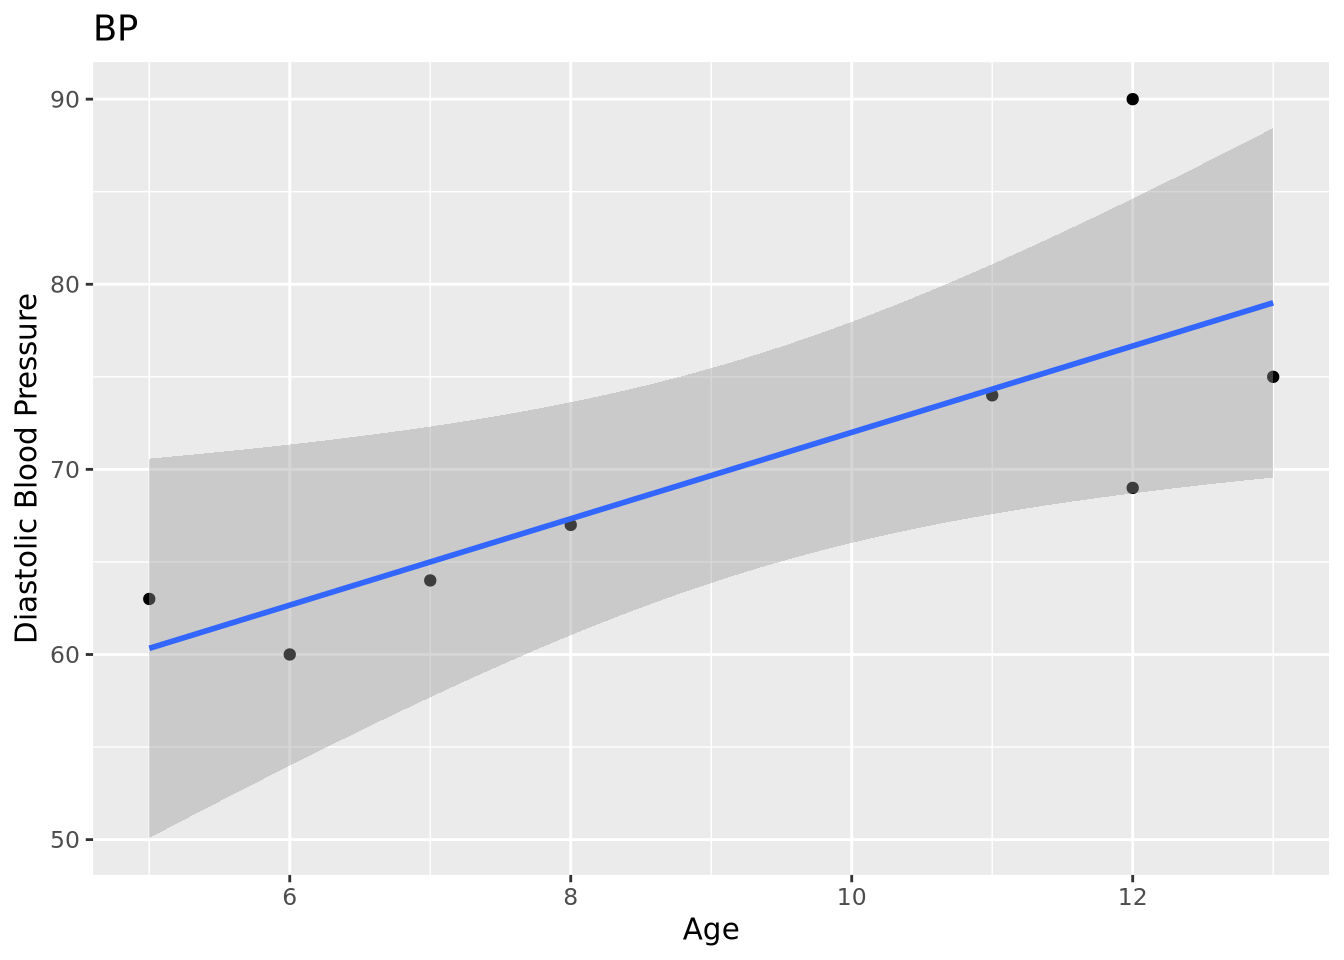
\includegraphics{Delete_files/figure-latex/unnamed-chunk-3-1.pdf} The
estimated regressio function is Y = 48.6667 + 2.3333(Age)

\begin{enumerate}
\def\labelenumi{(\alph{enumi})}
\setcounter{enumi}{1}
\tightlist
\item
  Plot the residuals ei against Xi. What does your residual plot show?
\end{enumerate}

\begin{Shaded}
\begin{Highlighting}[]
\FunctionTok{ggplot}\NormalTok{(bp\_lm, }\FunctionTok{aes}\NormalTok{(}\AttributeTok{x =}\NormalTok{ Age, }\AttributeTok{y =}\NormalTok{ .resid)) }\SpecialCharTok{+} \FunctionTok{geom\_point}\NormalTok{(}\AttributeTok{color =} \StringTok{"blue"}\NormalTok{, }\AttributeTok{dotsize =}\NormalTok{ .}\DecValTok{5}\NormalTok{) }\SpecialCharTok{+} \FunctionTok{theme\_bw}\NormalTok{()}
\end{Highlighting}
\end{Shaded}

\begin{verbatim}
## Warning in geom_point(color = "blue", dotsize = 0.5): Ignoring unknown
## parameters: `dotsize`
\end{verbatim}

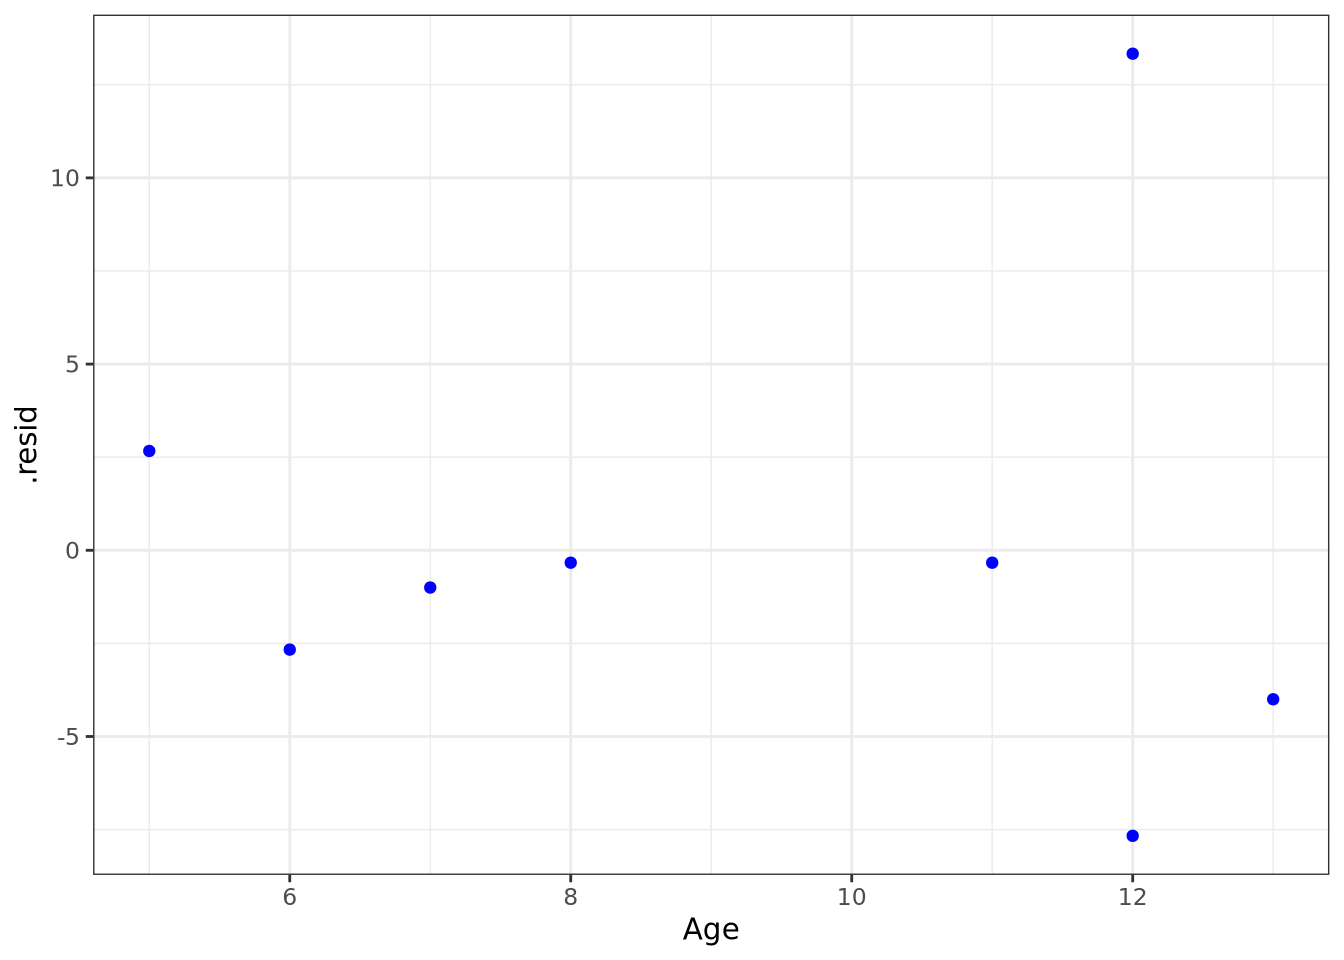
\includegraphics{Delete_files/figure-latex/unnamed-chunk-4-1.pdf} The
plot shows that case 7 is an outlier, having a residual of nearly 15,
while all of the other points appear to line up much closer to their
expected values.

\begin{enumerate}
\def\labelenumi{(\alph{enumi})}
\setcounter{enumi}{2}
\tightlist
\item
  Omit case 7 from the data and obtain the estimated regression function
  based on the remaining seven cases.
\end{enumerate}

\begin{Shaded}
\begin{Highlighting}[]
\NormalTok{xi2 }\OtherTok{\textless{}{-}} \FunctionTok{c}\NormalTok{(}\DecValTok{5}\NormalTok{, }\DecValTok{8}\NormalTok{, }\DecValTok{11}\NormalTok{, }\DecValTok{7}\NormalTok{, }\DecValTok{13}\NormalTok{, }\DecValTok{12}\NormalTok{, }\DecValTok{6}\NormalTok{)}
\NormalTok{yi2 }\OtherTok{\textless{}{-}} \FunctionTok{c}\NormalTok{(}\DecValTok{63}\NormalTok{, }\DecValTok{67}\NormalTok{, }\DecValTok{74}\NormalTok{, }\DecValTok{64}\NormalTok{, }\DecValTok{75}\NormalTok{, }\DecValTok{69}\NormalTok{, }\DecValTok{60}\NormalTok{)}
\NormalTok{bp2 }\OtherTok{\textless{}{-}} \FunctionTok{data.frame}\NormalTok{(xi2,yi2)}
\FunctionTok{colnames}\NormalTok{(bp2) }\OtherTok{\textless{}{-}} \FunctionTok{c}\NormalTok{(}\StringTok{"Age"}\NormalTok{, }\StringTok{"DBP"}\NormalTok{)}
\NormalTok{bp2}
\end{Highlighting}
\end{Shaded}

\begin{verbatim}
##   Age DBP
## 1   5  63
## 2   8  67
## 3  11  74
## 4   7  64
## 5  13  75
## 6  12  69
## 7   6  60
\end{verbatim}

\begin{Shaded}
\begin{Highlighting}[]
\NormalTok{n }\OtherTok{\textless{}{-}} \FunctionTok{nrow}\NormalTok{(bp2)}

\NormalTok{X }\OtherTok{\textless{}{-}}\NormalTok{ bp2}\SpecialCharTok{$}\NormalTok{Age}
\NormalTok{Y }\OtherTok{\textless{}{-}}\NormalTok{ bp2}\SpecialCharTok{$}\NormalTok{DBP}
\NormalTok{Y }\OtherTok{\textless{}{-}} \FunctionTok{as.matrix}\NormalTok{(Y)}
\NormalTok{Y}
\end{Highlighting}
\end{Shaded}

\begin{verbatim}
##      [,1]
## [1,]   63
## [2,]   67
## [3,]   74
## [4,]   64
## [5,]   75
## [6,]   69
## [7,]   60
\end{verbatim}

\begin{Shaded}
\begin{Highlighting}[]
\NormalTok{X }\OtherTok{\textless{}{-}} \FunctionTok{as.matrix}\NormalTok{(X)}
\NormalTok{X }\OtherTok{\textless{}{-}} \FunctionTok{cbind}\NormalTok{(}\FunctionTok{rep}\NormalTok{(}\DecValTok{1}\NormalTok{,n), X)}
\NormalTok{X}
\end{Highlighting}
\end{Shaded}

\begin{verbatim}
##      [,1] [,2]
## [1,]    1    5
## [2,]    1    8
## [3,]    1   11
## [4,]    1    7
## [5,]    1   13
## [6,]    1   12
## [7,]    1    6
\end{verbatim}

\begin{Shaded}
\begin{Highlighting}[]
\NormalTok{bp2\_lm }\OtherTok{\textless{}{-}} \FunctionTok{lm}\NormalTok{(DBP }\SpecialCharTok{\textasciitilde{}}\NormalTok{ Age, }\AttributeTok{data =}\NormalTok{ bp2)}
\FunctionTok{summary}\NormalTok{(bp2\_lm)}
\end{Highlighting}
\end{Shaded}

\begin{verbatim}
## 
## Call:
## lm(formula = DBP ~ Age, data = bp2)
## 
## Residuals:
##       1       2       3       4       5       6       7 
##  1.8252  0.9612  3.0971 -0.4175  0.8544 -3.5243 -2.7961 
## 
## Coefficients:
##             Estimate Std. Error t value Pr(>|t|)    
## (Intercept)  53.0680     3.2136  16.514 1.49e-05 ***
## Age           1.6214     0.3448   4.702  0.00533 ** 
## ---
## Signif. codes:  0 '***' 0.001 '**' 0.01 '*' 0.05 '.' 0.1 ' ' 1
## 
## Residual standard error: 2.645 on 5 degrees of freedom
## Multiple R-squared:  0.8156, Adjusted R-squared:  0.7787 
## F-statistic: 22.11 on 1 and 5 DF,  p-value: 0.005327
\end{verbatim}

\begin{Shaded}
\begin{Highlighting}[]
\FunctionTok{library}\NormalTok{(ggplot2)}

\FunctionTok{ggplot}\NormalTok{(bp2, }\FunctionTok{aes}\NormalTok{(}\AttributeTok{x =}\NormalTok{ Age, }\AttributeTok{y =}\NormalTok{ DBP)) }\SpecialCharTok{+}
  \FunctionTok{geom\_point}\NormalTok{() }\SpecialCharTok{+}
  \FunctionTok{labs}\NormalTok{(}\AttributeTok{x =} \StringTok{"Age"}\NormalTok{, }\AttributeTok{y =} \StringTok{"Diastolic Blood Pressure"}\NormalTok{, }\AttributeTok{title =} \StringTok{"BP"}\NormalTok{) }\SpecialCharTok{+}
  \FunctionTok{geom\_smooth}\NormalTok{(}\AttributeTok{method =}\NormalTok{ lm)}
\end{Highlighting}
\end{Shaded}

\begin{verbatim}
## `geom_smooth()` using formula = 'y ~ x'
\end{verbatim}

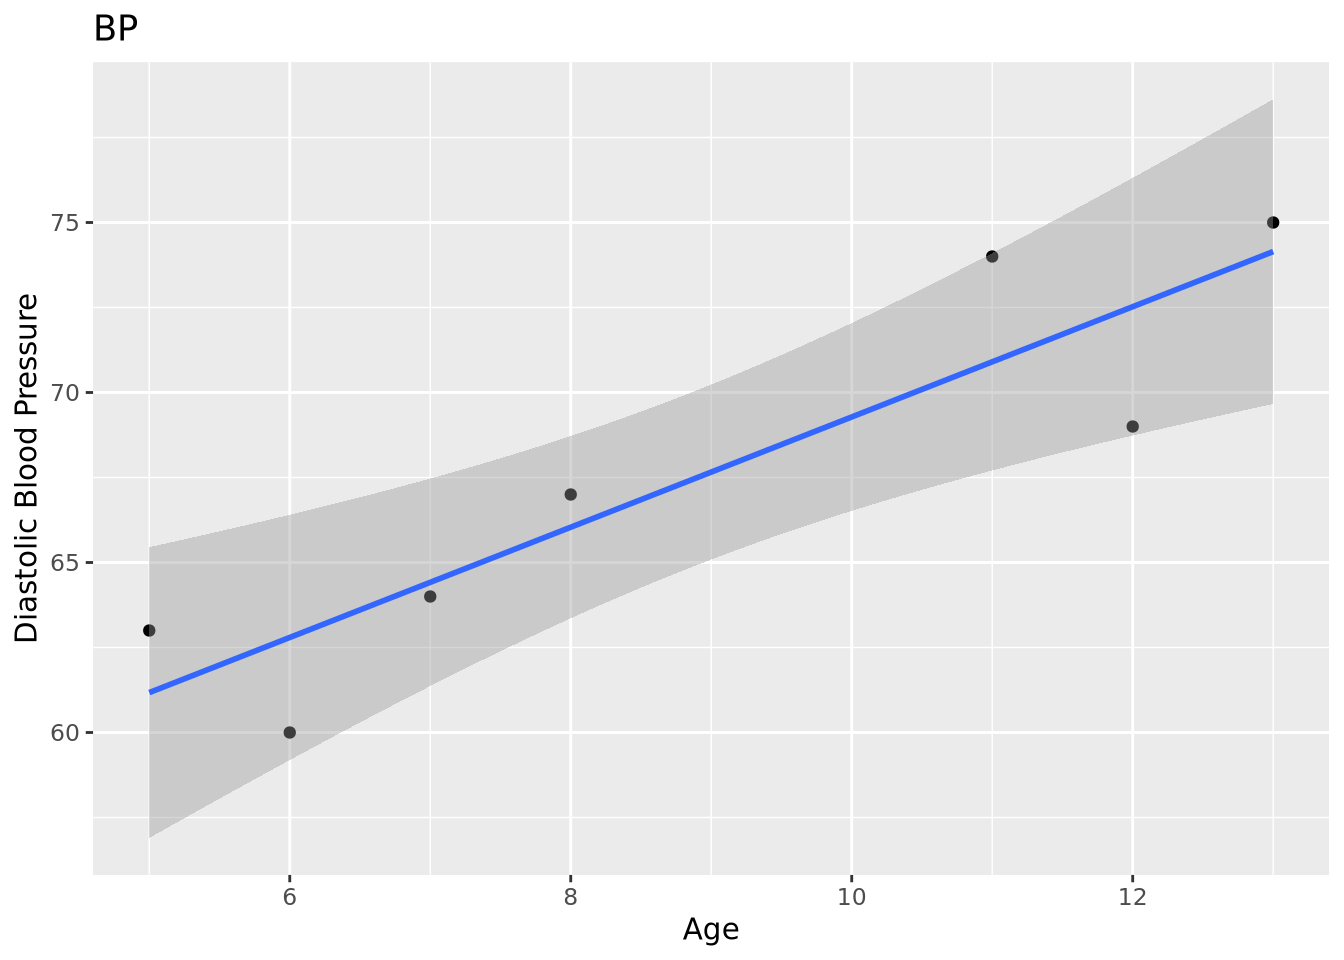
\includegraphics{Delete_files/figure-latex/unnamed-chunk-6-1.pdf}

\begin{enumerate}
\def\labelenumi{(\alph{enumi})}
\setcounter{enumi}{3}
\tightlist
\item
  Compare this estimated regression function to that obtained in part
  (a). What can you conclude about the effect of case 7?
\end{enumerate}

The model without case 7 is much more nicely fit to the expected data,
so we conclude that case 7 was a large outlier.

\begin{enumerate}
\def\labelenumi{(\alph{enumi})}
\setcounter{enumi}{4}
\tightlist
\item
  Using your fitted regression function in part (c), obtain a 99 percent
  predictioninterval for a new Y observation at X = 12. Does observation
  Y7 fall outside this prediction interval? What is the significance of
  this?
\end{enumerate}

\begin{Shaded}
\begin{Highlighting}[]
\NormalTok{xnew }\OtherTok{\textless{}{-}} \FunctionTok{t}\NormalTok{(}\FunctionTok{c}\NormalTok{(}\AttributeTok{Age =} \DecValTok{12}\NormalTok{, }\AttributeTok{DBP =} \FloatTok{72.525}\NormalTok{))}
\NormalTok{xnew }\OtherTok{\textless{}{-}} \FunctionTok{data.frame}\NormalTok{(xnew)}
\NormalTok{xnew}
\end{Highlighting}
\end{Shaded}

\begin{verbatim}
##   Age    DBP
## 1  12 72.525
\end{verbatim}

\begin{Shaded}
\begin{Highlighting}[]
\FunctionTok{predict}\NormalTok{(bp2\_lm, xnew, }\AttributeTok{interval =} \StringTok{"pred"}\NormalTok{,}\AttributeTok{level =}\NormalTok{ .}\DecValTok{99}\NormalTok{)}
\end{Highlighting}
\end{Shaded}

\begin{verbatim}
##        fit      lwr      upr
## 1 72.52427 60.31266 84.73588
\end{verbatim}

Observation Y7 falls outside of the 99\% prediction interval, which
indcates that this obervation is much higher than in should be based on
the estimated regresion function.

\begin{enumerate}
\def\labelenumi{\arabic{enumi})}
\setcounter{enumi}{2}
\tightlist
\item
  A chemist studied the concentration of a solution (Y) over time (X).
  Fifteen identical solutions were prepared. The 15 solutions were
  randomly divided into five sets of three, and the five sets were
  measured, respectively, after 1, 3, 5, 7, and 9 hours. The results
  follow.
\end{enumerate}

\begin{Shaded}
\begin{Highlighting}[]
\NormalTok{xi }\OtherTok{\textless{}{-}} \FunctionTok{c}\NormalTok{(}\DecValTok{9}\NormalTok{, }\DecValTok{9}\NormalTok{, }\DecValTok{9}\NormalTok{, }\DecValTok{7}\NormalTok{, }\DecValTok{7}\NormalTok{, }\DecValTok{7}\NormalTok{, }\DecValTok{5}\NormalTok{, }\DecValTok{5}\NormalTok{, }\DecValTok{5}\NormalTok{, }\DecValTok{3}\NormalTok{, }\DecValTok{3}\NormalTok{, }\DecValTok{3}\NormalTok{, }\DecValTok{1}\NormalTok{, }\DecValTok{1}\NormalTok{, }\DecValTok{1}\NormalTok{)}
\NormalTok{yi }\OtherTok{\textless{}{-}} \FunctionTok{c}\NormalTok{(}\FloatTok{0.07}\NormalTok{, }\FloatTok{0.09}\NormalTok{, }\FloatTok{0.08}\NormalTok{, }\FloatTok{0.16}\NormalTok{, }\FloatTok{0.17}\NormalTok{, }\FloatTok{0.21}\NormalTok{, }\FloatTok{0.49}\NormalTok{, }\FloatTok{0.58}\NormalTok{, }\FloatTok{0.53}\NormalTok{, }\FloatTok{1.22}\NormalTok{, }\FloatTok{1.15}\NormalTok{, }\FloatTok{1.07}\NormalTok{, }\FloatTok{2.84}\NormalTok{, }\FloatTok{2.57}\NormalTok{, }\FloatTok{3.10}\NormalTok{)}
\NormalTok{solution }\OtherTok{\textless{}{-}} \FunctionTok{data.frame}\NormalTok{(xi,yi)}
\FunctionTok{colnames}\NormalTok{(solution) }\OtherTok{\textless{}{-}} \FunctionTok{c}\NormalTok{(}\StringTok{"Time"}\NormalTok{, }\StringTok{"Concentration"}\NormalTok{)}
\NormalTok{solution}
\end{Highlighting}
\end{Shaded}

\begin{verbatim}
##    Time Concentration
## 1     9          0.07
## 2     9          0.09
## 3     9          0.08
## 4     7          0.16
## 5     7          0.17
## 6     7          0.21
## 7     5          0.49
## 8     5          0.58
## 9     5          0.53
## 10    3          1.22
## 11    3          1.15
## 12    3          1.07
## 13    1          2.84
## 14    1          2.57
## 15    1          3.10
\end{verbatim}

\begin{Shaded}
\begin{Highlighting}[]
\NormalTok{n }\OtherTok{\textless{}{-}} \FunctionTok{nrow}\NormalTok{(solution)}
\end{Highlighting}
\end{Shaded}

\begin{Shaded}
\begin{Highlighting}[]
\NormalTok{X }\OtherTok{\textless{}{-}}\NormalTok{ solution}\SpecialCharTok{$}\NormalTok{Time}
\NormalTok{Y }\OtherTok{\textless{}{-}}\NormalTok{ solution}\SpecialCharTok{$}\NormalTok{Concentration}
\NormalTok{Y }\OtherTok{\textless{}{-}} \FunctionTok{as.matrix}\NormalTok{(Y)}
\NormalTok{Y}
\end{Highlighting}
\end{Shaded}

\begin{verbatim}
##       [,1]
##  [1,] 0.07
##  [2,] 0.09
##  [3,] 0.08
##  [4,] 0.16
##  [5,] 0.17
##  [6,] 0.21
##  [7,] 0.49
##  [8,] 0.58
##  [9,] 0.53
## [10,] 1.22
## [11,] 1.15
## [12,] 1.07
## [13,] 2.84
## [14,] 2.57
## [15,] 3.10
\end{verbatim}

\begin{Shaded}
\begin{Highlighting}[]
\NormalTok{X }\OtherTok{\textless{}{-}} \FunctionTok{as.matrix}\NormalTok{(X)}
\NormalTok{X }\OtherTok{\textless{}{-}} \FunctionTok{cbind}\NormalTok{(}\FunctionTok{rep}\NormalTok{(}\DecValTok{1}\NormalTok{,n), X)}
\NormalTok{X}
\end{Highlighting}
\end{Shaded}

\begin{verbatim}
##       [,1] [,2]
##  [1,]    1    9
##  [2,]    1    9
##  [3,]    1    9
##  [4,]    1    7
##  [5,]    1    7
##  [6,]    1    7
##  [7,]    1    5
##  [8,]    1    5
##  [9,]    1    5
## [10,]    1    3
## [11,]    1    3
## [12,]    1    3
## [13,]    1    1
## [14,]    1    1
## [15,]    1    1
\end{verbatim}

\begin{enumerate}
\def\labelenumi{(\alph{enumi})}
\tightlist
\item
  Prepare a scatter plot of the data. What transformation of Y might you
  try, usingthe prototype patterns learned in class to achieve constant
  variance and linearity?
\end{enumerate}

\begin{Shaded}
\begin{Highlighting}[]
\NormalTok{solution\_lm }\OtherTok{\textless{}{-}} \FunctionTok{lm}\NormalTok{(Concentration }\SpecialCharTok{\textasciitilde{}}\NormalTok{ Time, }\AttributeTok{data =}\NormalTok{ solution)}
\FunctionTok{summary}\NormalTok{(solution\_lm)}
\end{Highlighting}
\end{Shaded}

\begin{verbatim}
## 
## Call:
## lm(formula = Concentration ~ Time, data = solution)
## 
## Residuals:
##     Min      1Q  Median      3Q     Max 
## -0.5333 -0.4043 -0.1373  0.4157  0.8487 
## 
## Coefficients:
##             Estimate Std. Error t value Pr(>|t|)    
## (Intercept)   2.5753     0.2487  10.354 1.20e-07 ***
## Time         -0.3240     0.0433  -7.483 4.61e-06 ***
## ---
## Signif. codes:  0 '***' 0.001 '**' 0.01 '*' 0.05 '.' 0.1 ' ' 1
## 
## Residual standard error: 0.4743 on 13 degrees of freedom
## Multiple R-squared:  0.8116, Adjusted R-squared:  0.7971 
## F-statistic: 55.99 on 1 and 13 DF,  p-value: 4.611e-06
\end{verbatim}

\begin{Shaded}
\begin{Highlighting}[]
\FunctionTok{ggplot}\NormalTok{(solution, }\FunctionTok{aes}\NormalTok{(}\AttributeTok{x =}\NormalTok{ Time, }\AttributeTok{y =}\NormalTok{ Concentration)) }\SpecialCharTok{+}
  \FunctionTok{geom\_point}\NormalTok{() }\SpecialCharTok{+}
  \FunctionTok{labs}\NormalTok{(}\AttributeTok{x =} \StringTok{"Time"}\NormalTok{, }\AttributeTok{y =} \StringTok{"Concentration"}\NormalTok{, }\AttributeTok{title =} \StringTok{"Solution"}\NormalTok{) }\SpecialCharTok{+}
  \FunctionTok{geom\_smooth}\NormalTok{(}\AttributeTok{method =}\NormalTok{ lm)}
\end{Highlighting}
\end{Shaded}

\begin{verbatim}
## `geom_smooth()` using formula = 'y ~ x'
\end{verbatim}

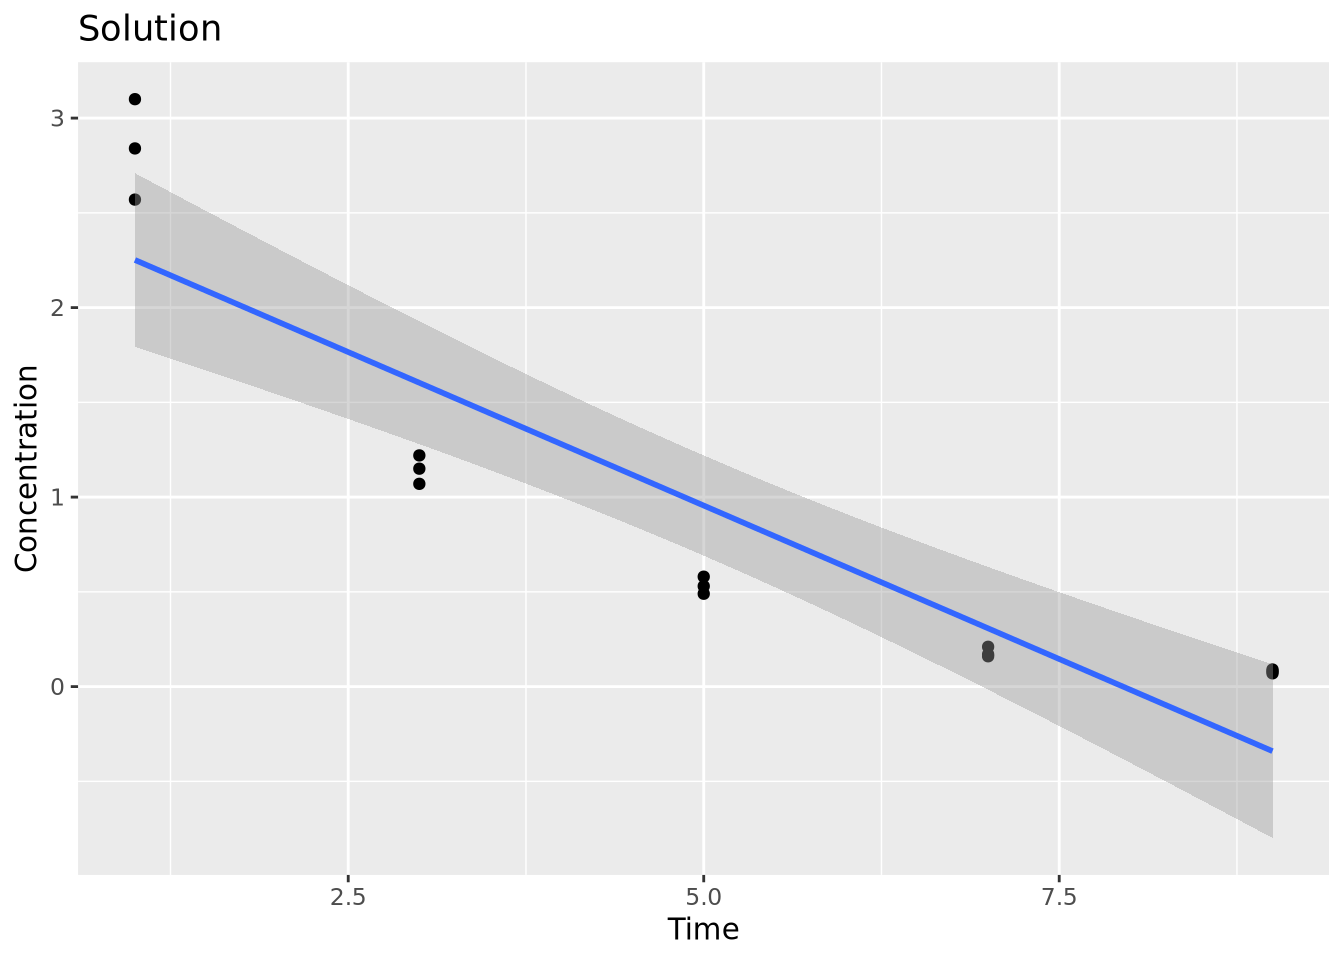
\includegraphics{Delete_files/figure-latex/unnamed-chunk-10-1.pdf} The
data appears to have a logarithmic or negative exponential relationship,
so such a transformation seems most appropriate.

\begin{enumerate}
\def\labelenumi{(\alph{enumi})}
\setcounter{enumi}{1}
\tightlist
\item
  Use the Box-Cox procedure and standardization to find an appropriate
  power transformation. Evaluate SSE for λ = −0.2, −0.1, 0, 0.1, 0.2
  What transformation of Y is suggested?
\end{enumerate}

\begin{Shaded}
\begin{Highlighting}[]
\FunctionTok{library}\NormalTok{(ALSM)}
\NormalTok{obj }\OtherTok{\textless{}{-}} \FunctionTok{boxcox.sse}\NormalTok{(solution}\SpecialCharTok{$}\NormalTok{Time, solution}\SpecialCharTok{$}\NormalTok{Concentration, }\AttributeTok{l=}\FunctionTok{seq}\NormalTok{(}\SpecialCharTok{{-}}\FloatTok{0.2}\NormalTok{, }\FloatTok{0.5}\NormalTok{, }\FloatTok{0.1}\NormalTok{))}
\end{Highlighting}
\end{Shaded}

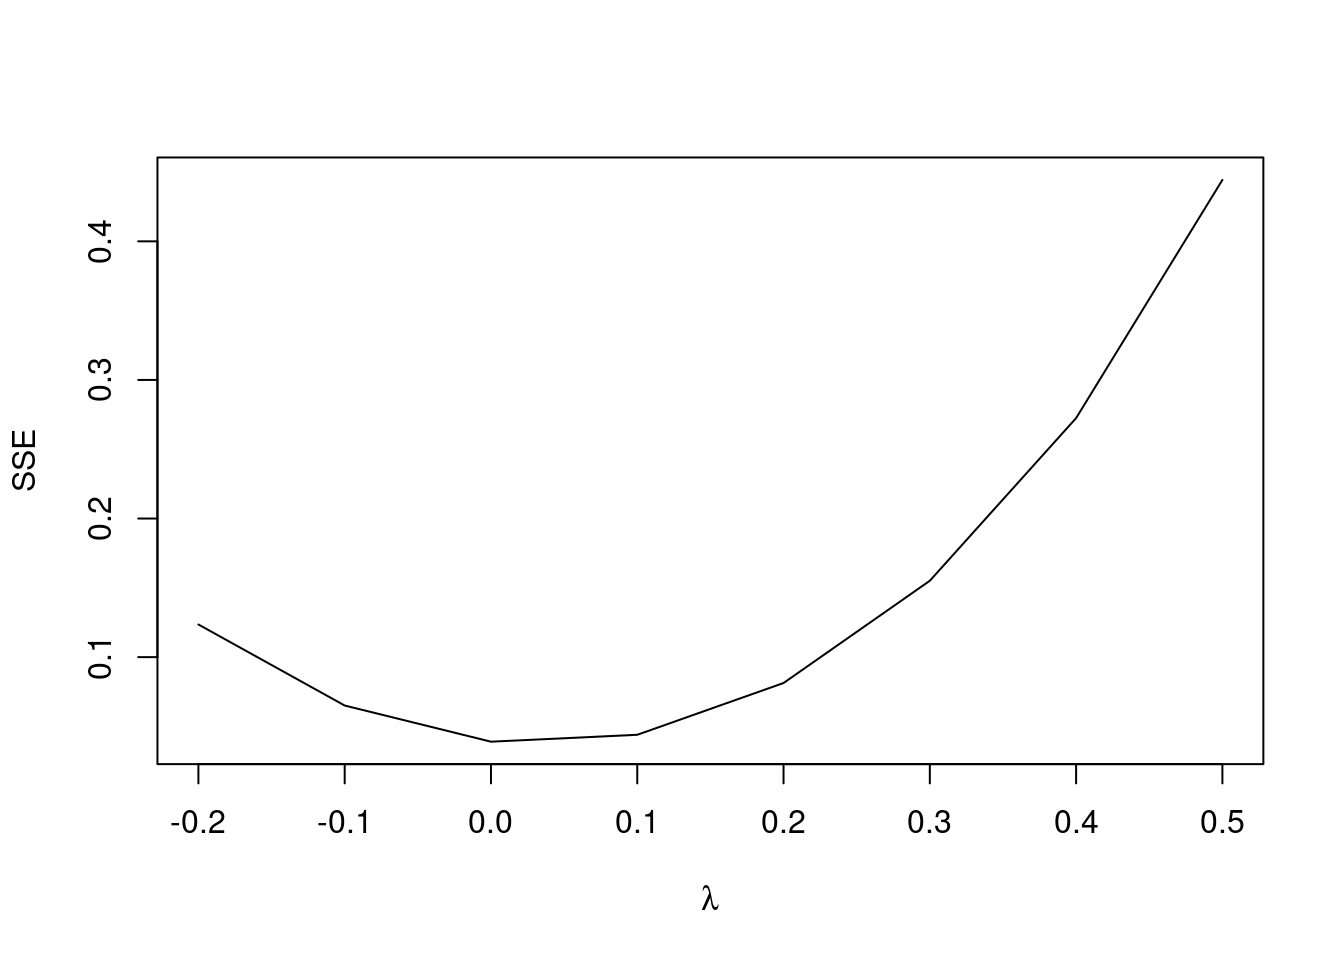
\includegraphics{Delete_files/figure-latex/unnamed-chunk-11-1.pdf}

\begin{Shaded}
\begin{Highlighting}[]
\NormalTok{obj}
\end{Highlighting}
\end{Shaded}

\begin{verbatim}
##   lambda        SSE
## 1   -0.2 0.12353047
## 2   -0.1 0.06505067
## 8    0.0 0.03897303
## 3    0.1 0.04396062
## 4    0.2 0.08131793
## 5    0.3 0.15509932
## 6    0.4 0.27246179
## 7    0.5 0.44429368
\end{verbatim}

We would select \(\lambda = 0.0\) since \(\lambda_{0.0} = 0.03897303\)
the minimum value.

\begin{enumerate}
\def\labelenumi{(\alph{enumi})}
\setcounter{enumi}{2}
\tightlist
\item
  Use the transformation Y0 = log10Y and obtain the estimated linear
  regression function for the transformed data.
\end{enumerate}

\begin{Shaded}
\begin{Highlighting}[]
\FunctionTok{library}\NormalTok{(dplyr)}

\NormalTok{solution }\OtherTok{\textless{}{-}}\NormalTok{ solution }\SpecialCharTok{\%\textgreater{}\%}
 \FunctionTok{mutate}\NormalTok{(}\AttributeTok{log10Y =} \FunctionTok{log10}\NormalTok{(Y))}
\NormalTok{log\_lm }\OtherTok{\textless{}{-}} \FunctionTok{lm}\NormalTok{(log10Y }\SpecialCharTok{\textasciitilde{}}\NormalTok{ X, solution)}
\NormalTok{log\_lm}
\end{Highlighting}
\end{Shaded}

\begin{verbatim}
## 
## Call:
## lm(formula = log10Y ~ X, data = solution)
## 
## Coefficients:
## (Intercept)           X1           X2  
##      0.6549           NA      -0.1954
\end{verbatim}

\begin{enumerate}
\def\labelenumi{(\alph{enumi})}
\setcounter{enumi}{3}
\tightlist
\item
  Plot the estimated regression line and the transformed data.
\end{enumerate}

\begin{Shaded}
\begin{Highlighting}[]
\CommentTok{\#ggplot(solution, aes(X, log10Y)) + geom\_point() + labs(x= "Time", y = "Concentration") + geom\_smooth(method = "lm", se = FALSE)}
\end{Highlighting}
\end{Shaded}

\begin{enumerate}
\def\labelenumi{(\alph{enumi})}
\setcounter{enumi}{4}
\tightlist
\item
  Does the regression line appear to be a good fit to the transformed
  data (Hint:perform a test to confirm your answer)?
\end{enumerate}

Yes, yet the code in the above problem no longer runs.

\begin{enumerate}
\def\labelenumi{(\alph{enumi})}
\setcounter{enumi}{5}
\tightlist
\item
  Obtain the residuals and plot them against the fitted values.
\end{enumerate}

\begin{Shaded}
\begin{Highlighting}[]
\FunctionTok{ggplot}\NormalTok{(solution\_lm, }\FunctionTok{aes}\NormalTok{(}\AttributeTok{x =}\NormalTok{ .fitted, }\AttributeTok{y =}\NormalTok{ .resid)) }\SpecialCharTok{+} \FunctionTok{geom\_point}\NormalTok{(}\AttributeTok{color =} \StringTok{"blue"}\NormalTok{, }\AttributeTok{dotsize =}\NormalTok{ .}\DecValTok{5}\NormalTok{) }\SpecialCharTok{+} \FunctionTok{theme\_bw}\NormalTok{()}
\end{Highlighting}
\end{Shaded}

\begin{verbatim}
## Warning in geom_point(color = "blue", dotsize = 0.5): Ignoring unknown
## parameters: `dotsize`
\end{verbatim}

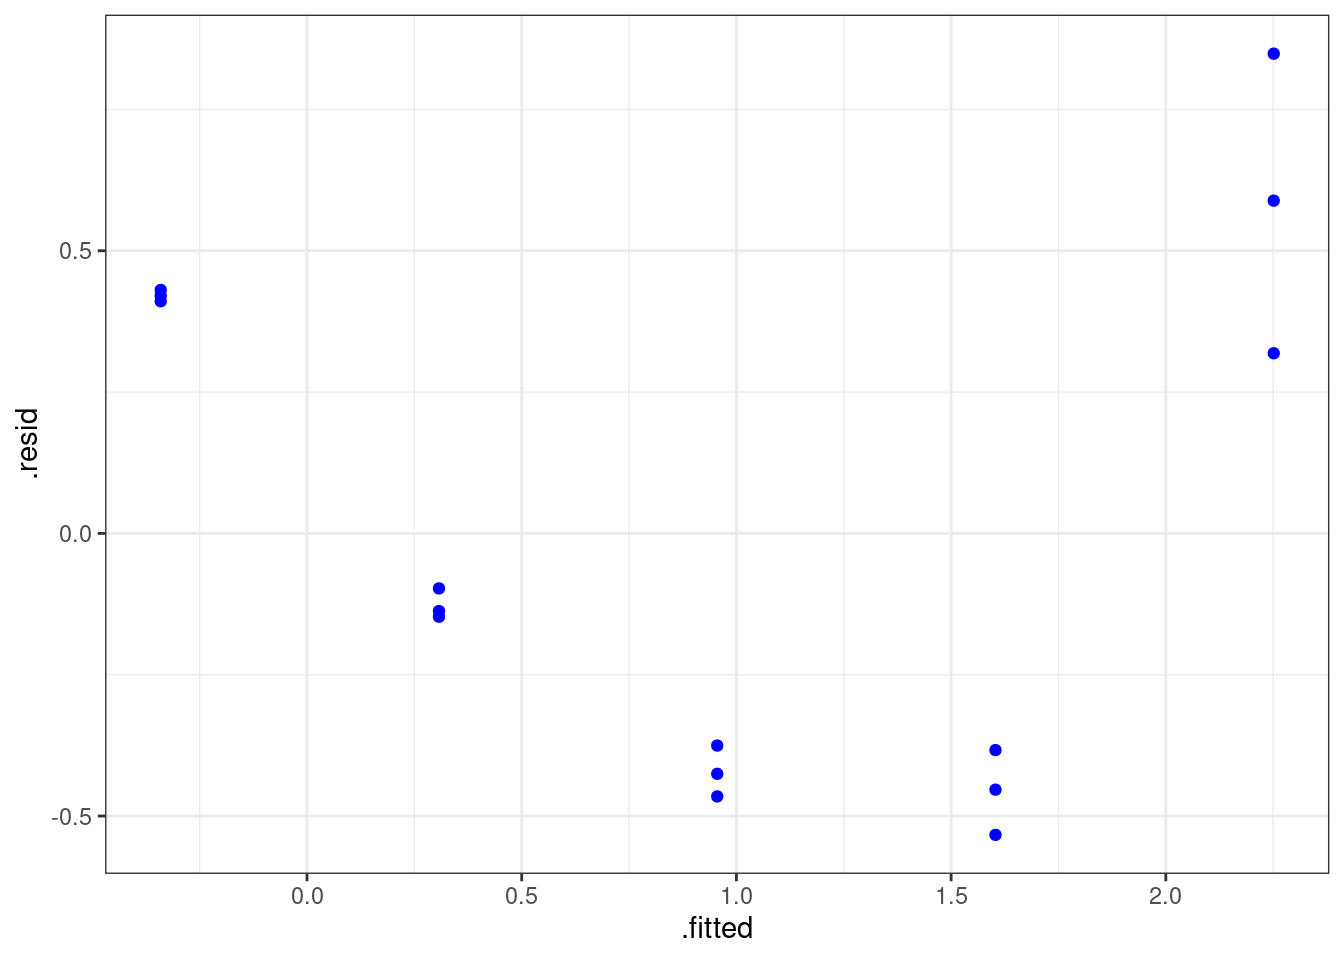
\includegraphics{Delete_files/figure-latex/unnamed-chunk-14-1.pdf}

\begin{enumerate}
\def\labelenumi{(\alph{enumi})}
\setcounter{enumi}{6}
\tightlist
\item
  Prepare a normal probability plot. What do your plots show?
\end{enumerate}

\begin{Shaded}
\begin{Highlighting}[]
\FunctionTok{ggplot}\NormalTok{(solution\_lm, }\FunctionTok{aes}\NormalTok{(}\AttributeTok{sample =}\NormalTok{ .resid)) }\SpecialCharTok{+} \FunctionTok{geom\_qq}\NormalTok{(}\AttributeTok{color =} \StringTok{"blue"}\NormalTok{) }\SpecialCharTok{+} \FunctionTok{geom\_qq\_line}\NormalTok{()}\SpecialCharTok{+} \FunctionTok{theme\_bw}\NormalTok{()}
\end{Highlighting}
\end{Shaded}

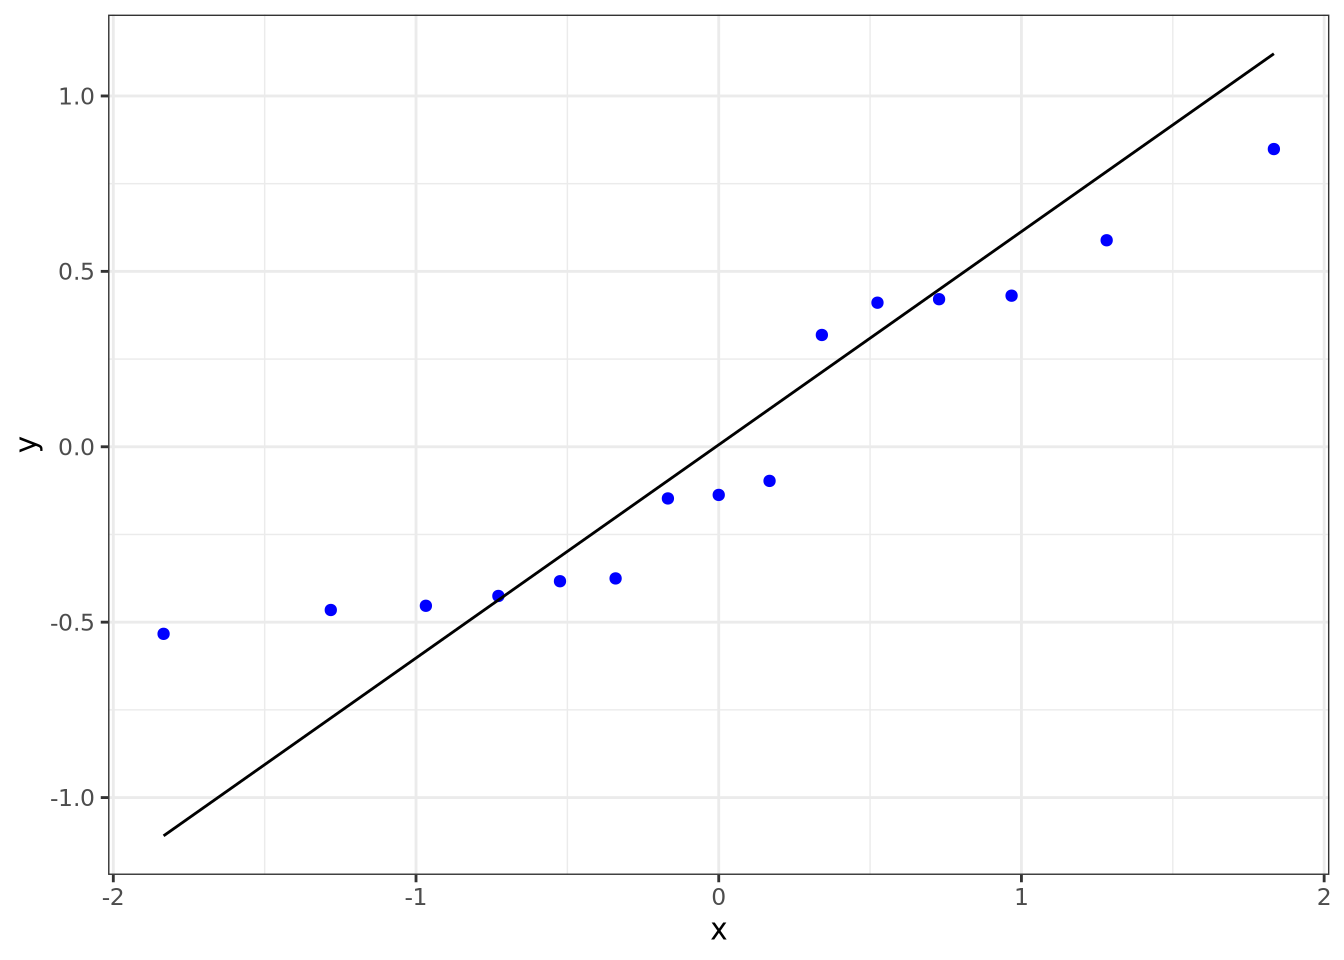
\includegraphics{Delete_files/figure-latex/unnamed-chunk-15-1.pdf}

\begin{enumerate}
\def\labelenumi{(\alph{enumi})}
\setcounter{enumi}{7}
\tightlist
\item
  Express the estimated regression function in the original units.
\end{enumerate}

Concentration = 2.5753 - 0.3240(Hours)

\url{http://www.cnachtsheim-text.csom.umn.edu/Kutner/Chapter\%20\%206\%20Data\%20Sets/CH06PR18.txt}

\begin{enumerate}
\def\labelenumi{\arabic{enumi})}
\setcounter{enumi}{3}
\tightlist
\item
\end{enumerate}

\begin{Shaded}
\begin{Highlighting}[]
\NormalTok{exam2 }\OtherTok{\textless{}{-}} \FunctionTok{read.table}\NormalTok{(}\StringTok{"http://users.stat.ufl.edu/\textasciitilde{}rrandles/sta4210/Rclassnotes/data/textdatasets/KutnerData/Chapter\%20\%206\%20Data\%20Sets/CH06PR18.txt"}\NormalTok{, }\AttributeTok{sep=}\StringTok{""}\NormalTok{, }\AttributeTok{header =} \ConstantTok{FALSE}\NormalTok{)}

\FunctionTok{colnames}\NormalTok{(exam2) }\OtherTok{\textless{}{-}} \FunctionTok{c}\NormalTok{(}\StringTok{"Y"}\NormalTok{, }\StringTok{"X1"}\NormalTok{, }\StringTok{"X2"}\NormalTok{, }\StringTok{"X3"}\NormalTok{, }\StringTok{"X4"}\NormalTok{)}

\NormalTok{exam2\_df }\OtherTok{\textless{}{-}} \FunctionTok{data.frame}\NormalTok{(exam2)}
\NormalTok{exam2}
\end{Highlighting}
\end{Shaded}

\begin{verbatim}
##         Y X1    X2   X3     X4
## 1  13.500  1  5.02 0.14 123000
## 2  12.000 14  8.19 0.27 104079
## 3  10.500 16  3.00 0.00  39998
## 4  15.000  4 10.70 0.05  57112
## 5  14.000 11  8.97 0.07  60000
## 6  10.500 15  9.45 0.24 101385
## 7  14.000  2  8.00 0.19  31300
## 8  16.500  1  6.62 0.60 248172
## 9  17.500  1  6.20 0.00 215000
## 10 16.500  8 11.78 0.03 251015
## 11 17.000 12 14.62 0.08 291264
## 12 16.500  2 11.55 0.03 207549
## 13 16.000  2  9.63 0.00  82000
## 14 16.500 13 12.99 0.04 359665
## 15 17.225  2 12.01 0.03 265500
## 16 17.000  1 12.01 0.00 299000
## 17 16.000  1  7.99 0.14 189258
## 18 14.625 12 10.33 0.12 366013
## 19 14.500 16 10.67 0.00 349930
## 20 14.500  3  9.45 0.03  85335
## 21 16.500  6 12.65 0.13 235932
## 22 16.500  3 12.08 0.00 130000
## 23 15.000  3 10.52 0.05  40500
## 24 15.000  3  9.47 0.00  40500
## 25 13.000 14 11.62 0.00  45959
## 26 12.500  1  5.00 0.33 120000
## 27 14.000 15  9.89 0.05  81243
## 28 13.750 16 11.13 0.06 153947
## 29 14.000  2  7.96 0.22  97321
## 30 15.000 16 10.73 0.09 276099
## 31 13.750  2  7.95 0.00  90000
## 32 15.625  3  9.10 0.00 184000
## 33 15.625  3 12.05 0.03 184718
## 34 13.000 16  8.43 0.04  96000
## 35 14.000 16 10.60 0.04 106350
## 36 15.250 13 10.55 0.10 135512
## 37 16.250  1  5.50 0.21 180000
## 38 13.000 14  8.53 0.03 315000
## 39 14.500  3  9.04 0.04  42500
## 40 11.500 15  8.20 0.00  30005
## 41 14.250  1  6.13 0.00  60000
## 42 15.500 15  8.32 0.00  73521
## 43 12.000  1  4.00 0.00  50000
## 44 14.250 15 10.10 0.00  50724
## 45 14.000  3  5.25 0.16  31750
## 46 16.500  3 11.62 0.00 168000
## 47 14.500  4  5.31 0.00  70000
## 48 15.500  1  5.75 0.00  27000
## 49 16.750  4 12.46 0.03 129614
## 50 16.750  4 12.75 0.00 129614
## 51 16.750  2 12.75 0.00 130000
## 52 16.750  2 11.38 0.00 209000
## 53 17.000  1  5.99 0.57 220000
## 54 16.000  2 11.37 0.27  60000
## 55 14.500  3 10.38 0.00 110000
## 56 15.000 15 10.77 0.05 101206
## 57 15.000 17 11.30 0.00 288847
## 58 16.000  1  7.06 0.14 105000
## 59 15.500 14 12.10 0.05 276425
## 60 15.250  2 10.04 0.06  33000
## 61 16.500  1  4.99 0.73 210000
## 62 19.250  0  7.33 0.22 240000
## 63 17.750 18 12.11 0.00 281552
## 64 18.750 16 12.86 0.00 421000
## 65 19.250 13 12.70 0.04 484290
## 66 14.000 20 11.58 0.00 234493
## 67 14.000 18 11.58 0.03 230675
## 68 18.000 16 12.97 0.08 296966
## 69 13.750  1  4.82 0.00  32000
## 70 15.000  2  9.75 0.03  38533
## 71 15.500 16 10.36 0.02 109912
## 72 15.900  1  8.13 0.23 236000
## 73 15.250 15 13.23 0.05 243338
## 74 15.500  4 10.57 0.04 122183
## 75 14.750 20 11.22 0.00 128268
## 76 15.000  3 10.34 0.00  72000
## 77 14.500  3 10.67 0.00  43404
## 78 13.500 18  8.60 0.08  59443
## 79 15.000 15 11.97 0.14 254700
## 80 15.250 11 11.27 0.03 434746
## 81 14.500 14 12.68 0.03 201930
\end{verbatim}

\begin{Shaded}
\begin{Highlighting}[]
\NormalTok{exam2\_lm }\OtherTok{\textless{}{-}} \FunctionTok{lm}\NormalTok{(Y }\SpecialCharTok{\textasciitilde{}}\NormalTok{ X1 }\SpecialCharTok{+}\NormalTok{ X2 }\SpecialCharTok{+}\NormalTok{ X3 }\SpecialCharTok{+}\NormalTok{ X4, }\AttributeTok{data =}\NormalTok{ exam2)}
\FunctionTok{summary}\NormalTok{(exam2\_lm)}
\end{Highlighting}
\end{Shaded}

\begin{verbatim}
## 
## Call:
## lm(formula = Y ~ X1 + X2 + X3 + X4, data = exam2)
## 
## Residuals:
##     Min      1Q  Median      3Q     Max 
## -3.1872 -0.5911 -0.0910  0.5579  2.9441 
## 
## Coefficients:
##               Estimate Std. Error t value Pr(>|t|)    
## (Intercept)  1.220e+01  5.780e-01  21.110  < 2e-16 ***
## X1          -1.420e-01  2.134e-02  -6.655 3.89e-09 ***
## X2           2.820e-01  6.317e-02   4.464 2.75e-05 ***
## X3           6.193e-01  1.087e+00   0.570     0.57    
## X4           7.924e-06  1.385e-06   5.722 1.98e-07 ***
## ---
## Signif. codes:  0 '***' 0.001 '**' 0.01 '*' 0.05 '.' 0.1 ' ' 1
## 
## Residual standard error: 1.137 on 76 degrees of freedom
## Multiple R-squared:  0.5847, Adjusted R-squared:  0.5629 
## F-statistic: 26.76 on 4 and 76 DF,  p-value: 7.272e-14
\end{verbatim}

\begin{enumerate}
\def\labelenumi{(\alph{enumi})}
\tightlist
\item
  Prepare a box plot for each predictor variable and prepare a grid of
  plot using the plot grid() function in the cowplot library.
\end{enumerate}

\begin{Shaded}
\begin{Highlighting}[]
\FunctionTok{library}\NormalTok{(cowplot)}
\NormalTok{X\_1 }\OtherTok{\textless{}{-}} \FunctionTok{ggplot}\NormalTok{(exam2\_lm, }\FunctionTok{aes}\NormalTok{(}\AttributeTok{x =}\NormalTok{ X1)) }\SpecialCharTok{+} \FunctionTok{geom\_boxplot}\NormalTok{(}\AttributeTok{color =} \StringTok{"steelblue"}\NormalTok{, }\AttributeTok{fill =} \StringTok{"orchid4"}\NormalTok{) }\SpecialCharTok{+} \FunctionTok{theme\_bw}\NormalTok{()}
\NormalTok{X\_2 }\OtherTok{\textless{}{-}} \FunctionTok{ggplot}\NormalTok{(exam2\_lm, }\FunctionTok{aes}\NormalTok{(}\AttributeTok{x =}\NormalTok{ X2)) }\SpecialCharTok{+} \FunctionTok{geom\_boxplot}\NormalTok{(}\AttributeTok{color =} \StringTok{"steelblue"}\NormalTok{, }\AttributeTok{fill =} \StringTok{"orchid4"}\NormalTok{) }\SpecialCharTok{+} \FunctionTok{theme\_bw}\NormalTok{()}
\NormalTok{X\_3 }\OtherTok{\textless{}{-}} \FunctionTok{ggplot}\NormalTok{(exam2\_lm, }\FunctionTok{aes}\NormalTok{(}\AttributeTok{x =}\NormalTok{ X3)) }\SpecialCharTok{+} \FunctionTok{geom\_boxplot}\NormalTok{(}\AttributeTok{color =} \StringTok{"steelblue"}\NormalTok{, }\AttributeTok{fill =} \StringTok{"orchid4"}\NormalTok{) }\SpecialCharTok{+} \FunctionTok{theme\_bw}\NormalTok{()}
\NormalTok{X\_4 }\OtherTok{\textless{}{-}} \FunctionTok{ggplot}\NormalTok{(exam2\_lm, }\FunctionTok{aes}\NormalTok{(}\AttributeTok{x =}\NormalTok{ X4)) }\SpecialCharTok{+} \FunctionTok{geom\_boxplot}\NormalTok{(}\AttributeTok{color =} \StringTok{"steelblue"}\NormalTok{, }\AttributeTok{fill =} \StringTok{"orchid4"}\NormalTok{) }\SpecialCharTok{+} \FunctionTok{theme\_bw}\NormalTok{()}

\FunctionTok{plot\_grid}\NormalTok{(X\_1, X\_2, X\_3, X\_4)}
\end{Highlighting}
\end{Shaded}

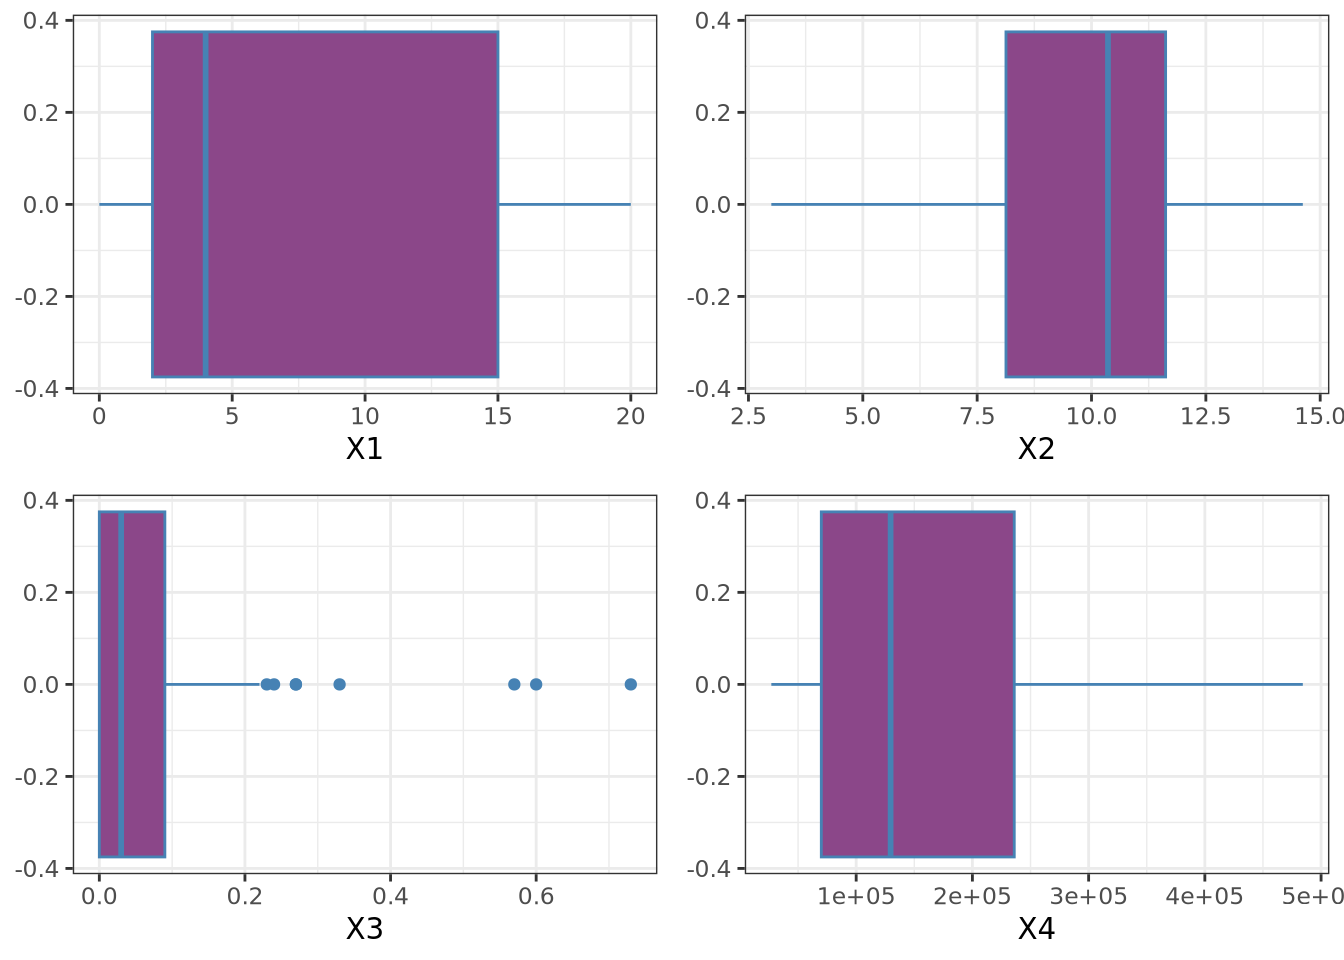
\includegraphics{Delete_files/figure-latex/unnamed-chunk-18-1.pdf}

\begin{enumerate}
\def\labelenumi{(\alph{enumi})}
\setcounter{enumi}{1}
\tightlist
\item
  What information do these plots provide?
\end{enumerate}

These plots show us the symmetry of the data per predictor variable,
whether or not it's skewed, if any potential outliers exist, the median,
and the interquartile range.

\begin{enumerate}
\def\labelenumi{(\alph{enumi})}
\setcounter{enumi}{2}
\tightlist
\item
  Obtain the scatter plot matrix and the correlation matrix.
\end{enumerate}

\begin{Shaded}
\begin{Highlighting}[]
\FunctionTok{colnames}\NormalTok{(exam2\_df) }\OtherTok{\textless{}{-}} \FunctionTok{c}\NormalTok{(}\StringTok{"Y"}\NormalTok{, }\StringTok{"X1"}\NormalTok{, }\StringTok{"X2"}\NormalTok{, }\StringTok{"X3"}\NormalTok{, }\StringTok{"X4"}\NormalTok{)}
\FunctionTok{pairs}\NormalTok{(exam2\_df)}
\end{Highlighting}
\end{Shaded}

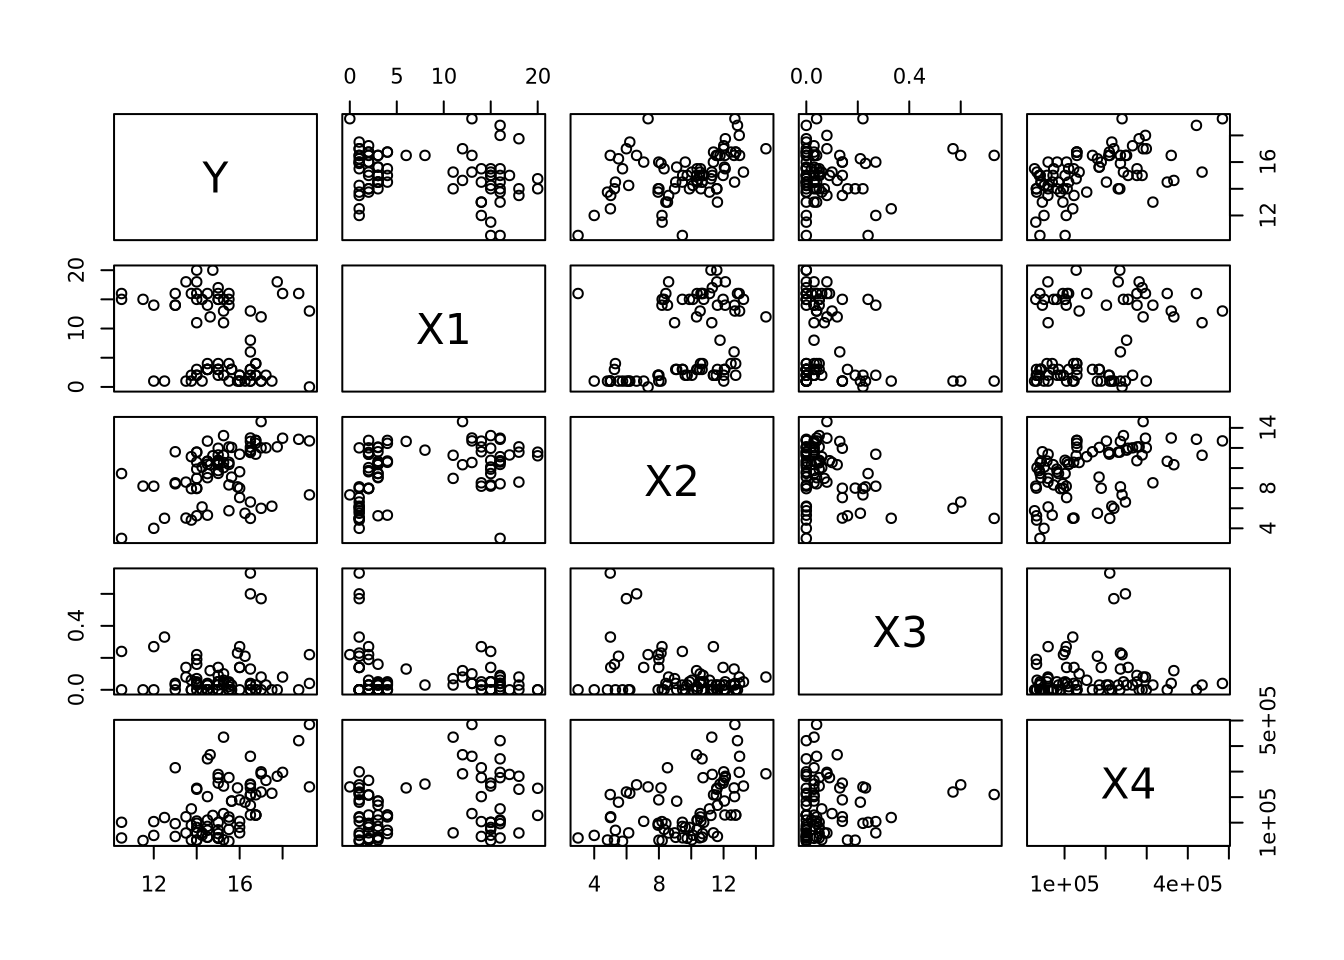
\includegraphics{Delete_files/figure-latex/unnamed-chunk-19-1.pdf}

\begin{Shaded}
\begin{Highlighting}[]
\FunctionTok{cor}\NormalTok{(exam2\_df)}
\end{Highlighting}
\end{Shaded}

\begin{verbatim}
##              Y         X1         X2          X3         X4
## Y   1.00000000 -0.2502846  0.4137872  0.06652647 0.53526237
## X1 -0.25028456  1.0000000  0.3888264 -0.25266347 0.28858350
## X2  0.41378716  0.3888264  1.0000000 -0.37976174 0.44069713
## X3  0.06652647 -0.2526635 -0.3797617  1.00000000 0.08061073
## X4  0.53526237  0.2885835  0.4406971  0.08061073 1.00000000
\end{verbatim}

\begin{enumerate}
\def\labelenumi{(\alph{enumi})}
\setcounter{enumi}{3}
\tightlist
\item
  Interpret these and state your principal findings in detail.
\end{enumerate}

The relationship between Y and X4 was the strongest of the 4, though
still only with a correlation coefficient of 0.53526237. The next
strongest relationship was Y and X2 with a correlation coefficient of
0.41378716. Y had very weak correlation to X3, and a weak negative
correlation with X1

\begin{enumerate}
\def\labelenumi{(\alph{enumi})}
\setcounter{enumi}{4}
\tightlist
\item
  Fit regression model for four predictor variables to the data. State
  the estimated regression function.
\end{enumerate}

\begin{Shaded}
\begin{Highlighting}[]
\NormalTok{exam2\_lm }\OtherTok{\textless{}{-}} \FunctionTok{lm}\NormalTok{(Y }\SpecialCharTok{\textasciitilde{}}\NormalTok{ X1 }\SpecialCharTok{+}\NormalTok{ X2 }\SpecialCharTok{+}\NormalTok{ X3 }\SpecialCharTok{+}\NormalTok{ X4, }\AttributeTok{data =}\NormalTok{ exam2)}
\FunctionTok{summary}\NormalTok{(exam2\_lm)}
\end{Highlighting}
\end{Shaded}

\begin{verbatim}
## 
## Call:
## lm(formula = Y ~ X1 + X2 + X3 + X4, data = exam2)
## 
## Residuals:
##     Min      1Q  Median      3Q     Max 
## -3.1872 -0.5911 -0.0910  0.5579  2.9441 
## 
## Coefficients:
##               Estimate Std. Error t value Pr(>|t|)    
## (Intercept)  1.220e+01  5.780e-01  21.110  < 2e-16 ***
## X1          -1.420e-01  2.134e-02  -6.655 3.89e-09 ***
## X2           2.820e-01  6.317e-02   4.464 2.75e-05 ***
## X3           6.193e-01  1.087e+00   0.570     0.57    
## X4           7.924e-06  1.385e-06   5.722 1.98e-07 ***
## ---
## Signif. codes:  0 '***' 0.001 '**' 0.01 '*' 0.05 '.' 0.1 ' ' 1
## 
## Residual standard error: 1.137 on 76 degrees of freedom
## Multiple R-squared:  0.5847, Adjusted R-squared:  0.5629 
## F-statistic: 26.76 on 4 and 76 DF,  p-value: 7.272e-14
\end{verbatim}

Y = 1.220e+01 - -1.420e-01(X1) + 2.820e-01(X2) + 6.193e-01(X3) +
7.924e-06(X4)

\begin{enumerate}
\def\labelenumi{(\alph{enumi})}
\setcounter{enumi}{5}
\tightlist
\item
  Obtain the residuals and prepare a box plot of the residuals.
\end{enumerate}

\begin{Shaded}
\begin{Highlighting}[]
\FunctionTok{ggplot}\NormalTok{(exam2\_lm, }\FunctionTok{aes}\NormalTok{(}\AttributeTok{x =}\NormalTok{ .fitted, }\AttributeTok{y =}\NormalTok{ .resid)) }\SpecialCharTok{+} \FunctionTok{geom\_point}\NormalTok{(}\AttributeTok{color =} \StringTok{"blue"}\NormalTok{, }\AttributeTok{dotsize =}\NormalTok{ .}\DecValTok{5}\NormalTok{) }\SpecialCharTok{+} \FunctionTok{theme\_bw}\NormalTok{()}
\end{Highlighting}
\end{Shaded}

\begin{verbatim}
## Warning in geom_point(color = "blue", dotsize = 0.5): Ignoring unknown
## parameters: `dotsize`
\end{verbatim}

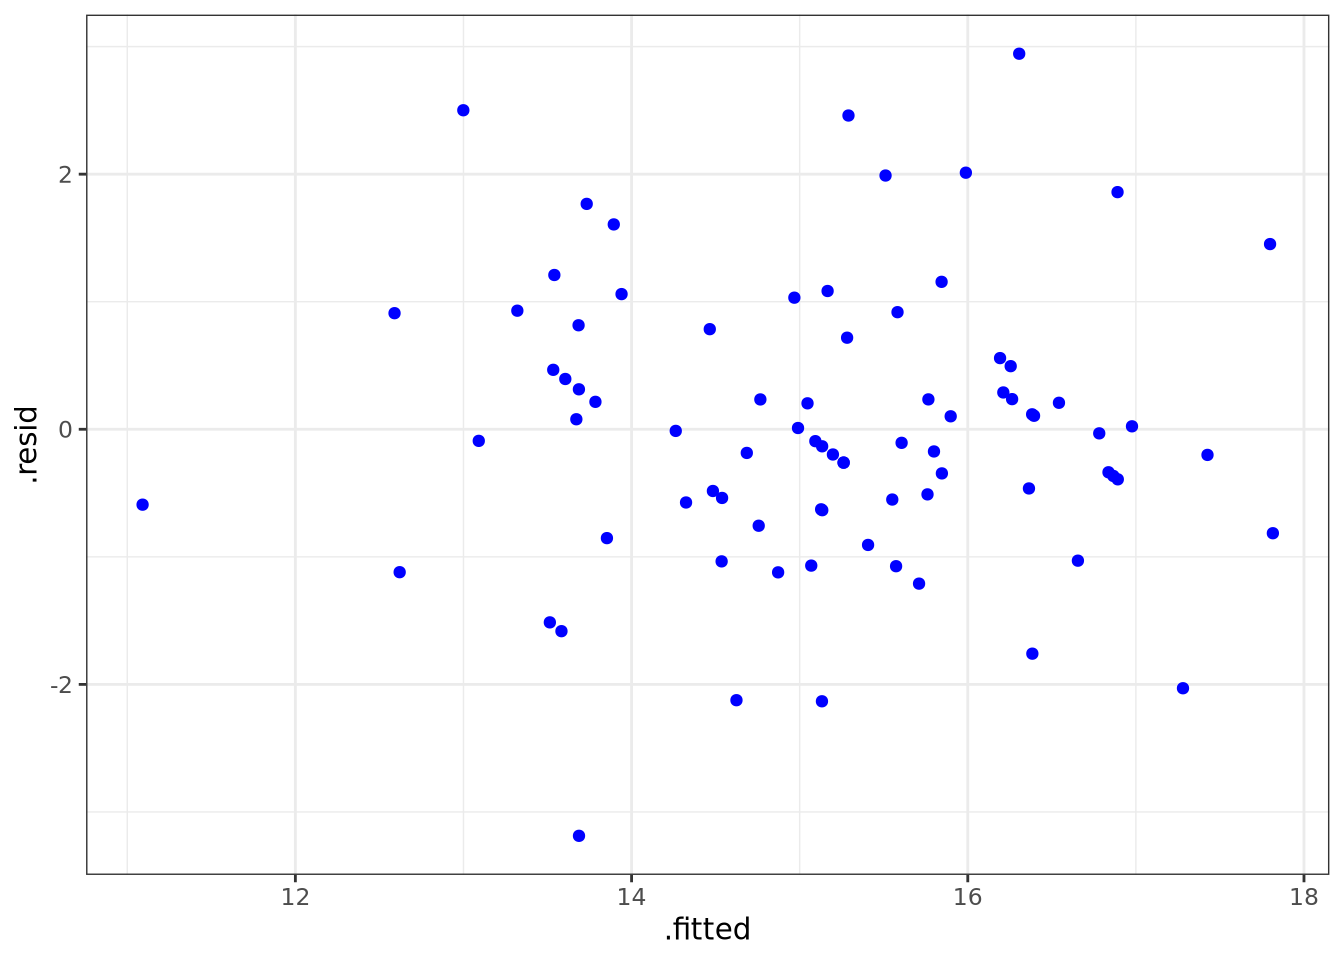
\includegraphics{Delete_files/figure-latex/unnamed-chunk-21-1.pdf}

\begin{Shaded}
\begin{Highlighting}[]
\FunctionTok{ggplot}\NormalTok{(exam2\_lm, }\FunctionTok{aes}\NormalTok{(}\AttributeTok{x =}\NormalTok{ .resid)) }\SpecialCharTok{+} \FunctionTok{geom\_boxplot}\NormalTok{(}\AttributeTok{color =} \StringTok{"steelblue"}\NormalTok{, }\AttributeTok{fill =} \StringTok{"orchid4"}\NormalTok{) }\SpecialCharTok{+} \FunctionTok{theme\_bw}\NormalTok{()}
\end{Highlighting}
\end{Shaded}

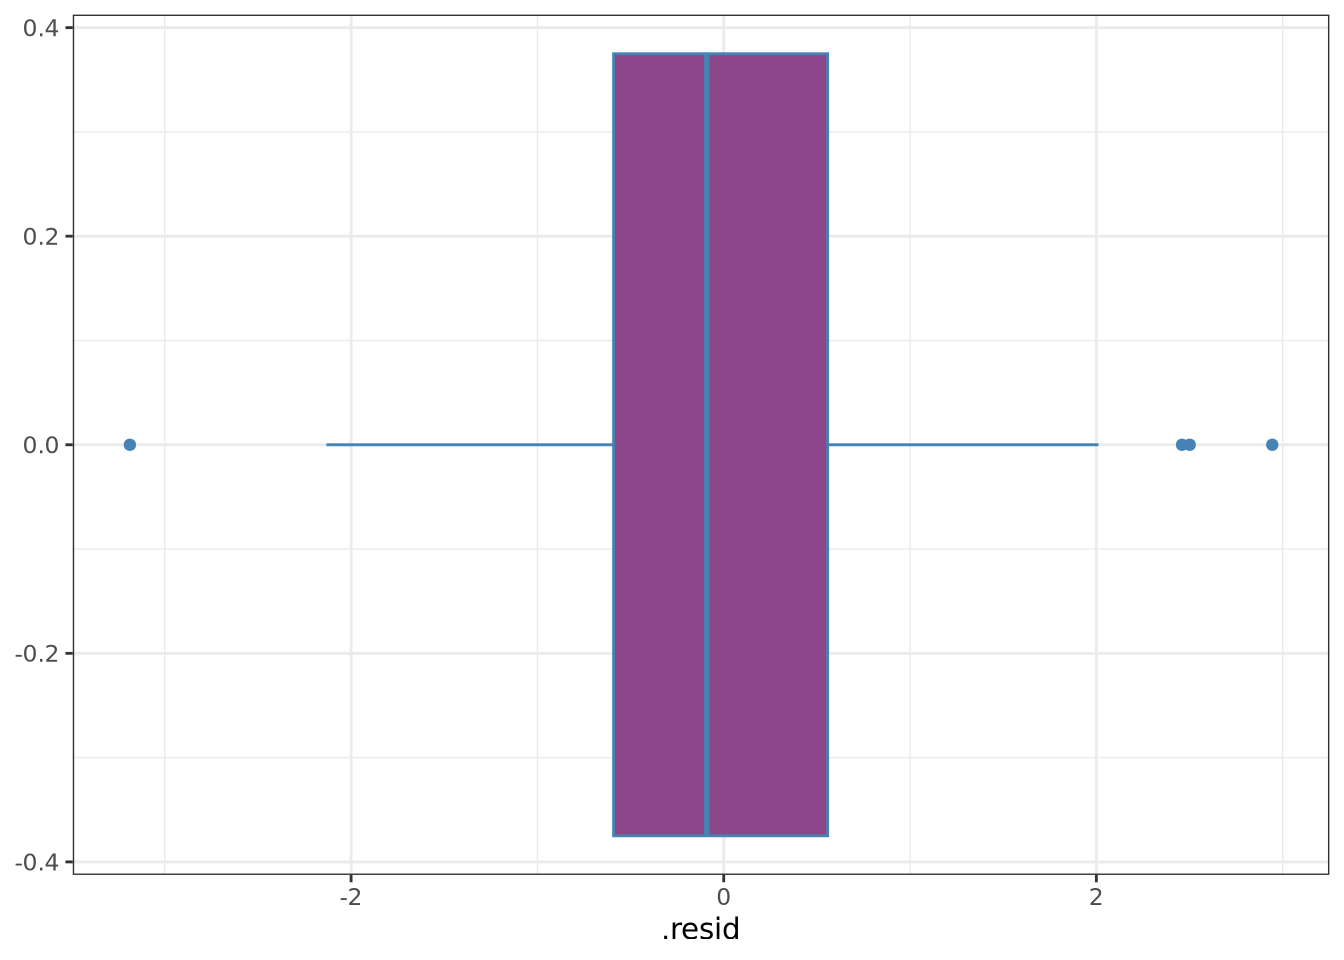
\includegraphics{Delete_files/figure-latex/unnamed-chunk-21-2.pdf}

\begin{enumerate}
\def\labelenumi{(\alph{enumi})}
\setcounter{enumi}{6}
\tightlist
\item
  Does the distribution appear to be fairly symmetrical?
\end{enumerate}

The distribution appears to be fairly symmetrical.

\begin{enumerate}
\def\labelenumi{(\alph{enumi})}
\setcounter{enumi}{7}
\tightlist
\item
  Plot the residuals against Yˆ , each predictor variable, and each
  two-factor interaction term on a grid of plot using the plot grid()
  function in the cowplot library.
\end{enumerate}

\begin{Shaded}
\begin{Highlighting}[]
\NormalTok{X\_1r }\OtherTok{\textless{}{-}} \FunctionTok{ggplot}\NormalTok{(exam2\_lm, }\FunctionTok{aes}\NormalTok{(}\AttributeTok{x =}\NormalTok{ X1, }\AttributeTok{y =}\NormalTok{ .resid)) }\SpecialCharTok{+} \FunctionTok{geom\_point}\NormalTok{() }\SpecialCharTok{+} \FunctionTok{theme\_bw}\NormalTok{()}
\NormalTok{X\_2r }\OtherTok{\textless{}{-}} \FunctionTok{ggplot}\NormalTok{(exam2\_lm, }\FunctionTok{aes}\NormalTok{(}\AttributeTok{x =}\NormalTok{ X2, }\AttributeTok{y =}\NormalTok{ .resid)) }\SpecialCharTok{+} \FunctionTok{geom\_point}\NormalTok{() }\SpecialCharTok{+} \FunctionTok{theme\_bw}\NormalTok{()}
\NormalTok{X\_3r }\OtherTok{\textless{}{-}} \FunctionTok{ggplot}\NormalTok{(exam2\_lm, }\FunctionTok{aes}\NormalTok{(}\AttributeTok{x =}\NormalTok{ X3, }\AttributeTok{y =}\NormalTok{ .resid)) }\SpecialCharTok{+} \FunctionTok{geom\_point}\NormalTok{() }\SpecialCharTok{+} \FunctionTok{theme\_bw}\NormalTok{()}
\NormalTok{X\_4r }\OtherTok{\textless{}{-}} \FunctionTok{ggplot}\NormalTok{(exam2\_lm, }\FunctionTok{aes}\NormalTok{(}\AttributeTok{x =}\NormalTok{ X4, }\AttributeTok{y =}\NormalTok{ .resid)) }\SpecialCharTok{+} \FunctionTok{geom\_point}\NormalTok{() }\SpecialCharTok{+} \FunctionTok{theme\_bw}\NormalTok{()}

\FunctionTok{plot\_grid}\NormalTok{(X\_1r, X\_2r, X\_3r, X\_4r)}
\end{Highlighting}
\end{Shaded}

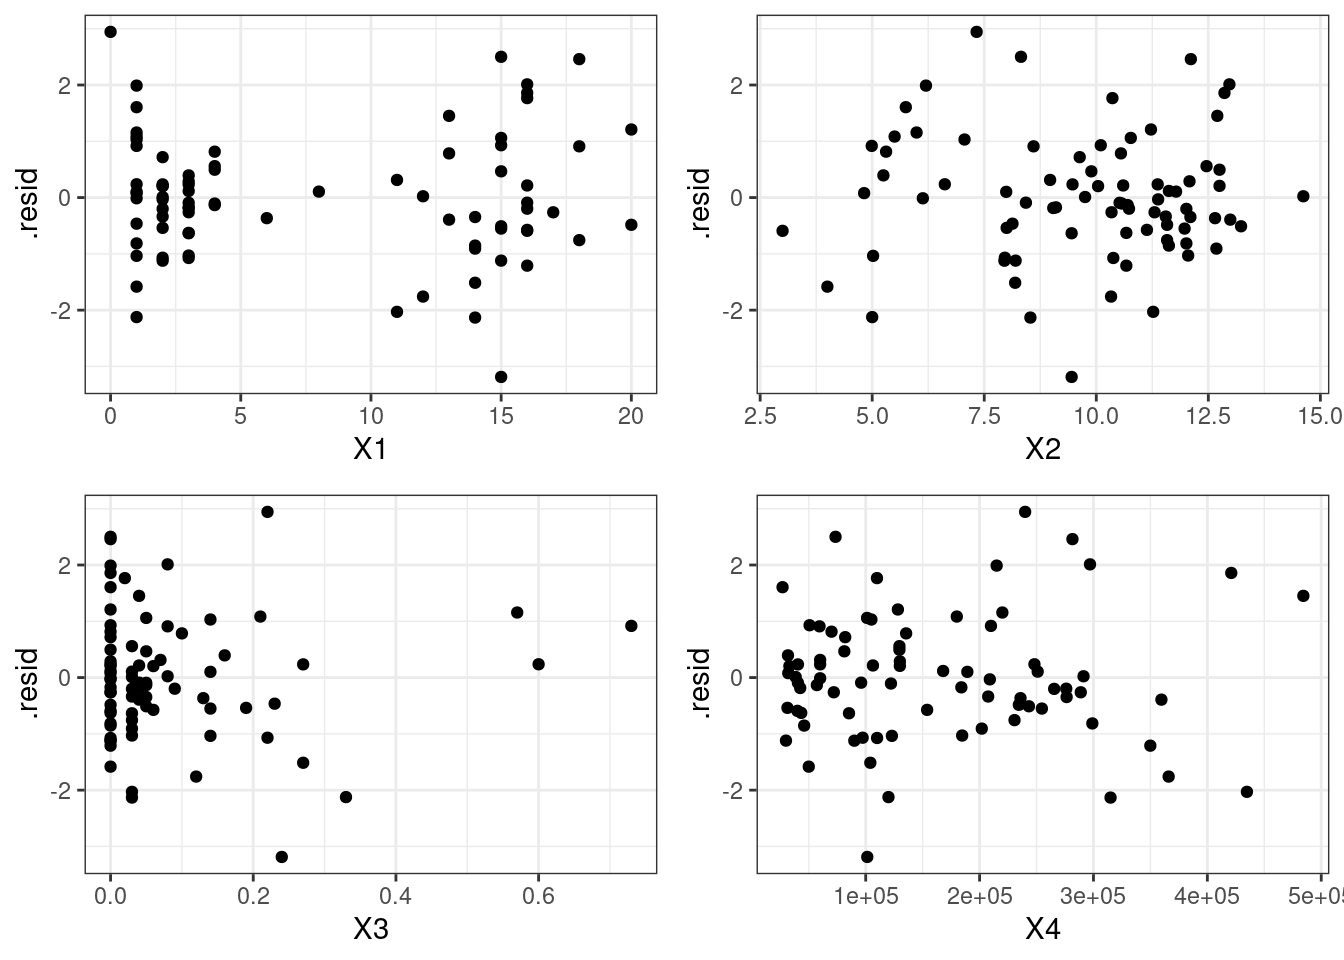
\includegraphics{Delete_files/figure-latex/unnamed-chunk-22-1.pdf}

\end{document}
